\documentclass[dvipdfmx]{jsarticle}
\usepackage[top=20truemm, bottom=20truemm, left=20truemm, right=20truemm]{geometry}
\usepackage{amsmath, amssymb, amsthm, mathtools, bm}
\usepackage[dvipdfmx]{graphicx}
\usepackage{subcaption}
\usepackage{float}
\usepackage{listings, jlisting}
\usepackage{color}
\usepackage{url}
\usepackage[dvipdfmx]{hyperref}
\usepackage{pxjahyper}
\usepackage{comment}

\theoremstyle{definition}
\newtheorem{definition}{定義}[section]
\newtheorem{theorem}[definition]{定理}
\newtheorem{example}[definition]{例}
\newtheorem{question}{問}[section]

\lstdefinelanguage{p5js}{
    morekeywords = [1]{  % keywords
        await, break, case, catch, class, const, continue, debugger, default, delete,
        do, else, enum, export, extends, finally, for, function, function*, if, implements, import, in,
        instanceof, interface, let, new, package, private, protected, public, return, static, super,
        switch, this, throw, try, typeof, var, void, while, with, yield, yield*
    },
    morekeywords = [2]{  % literal
        false, Infinity, NaN, null, true, undefined
    },
    morekeywords = [3] {  % Classes
        Array, ArrayBuffer, Boolean, DataView, Date, Error, EvalError, Float32Array, Float64Array,
        Function, Generator, GeneratorFunction, Int16Array, Int32Array, Int8Array, InternalError,
        JSON, Map, Math, Number, Object, Promise, Proxy, RangeError, ReferenceError, Reflect,
        RegExp, Set, String, Symbol, SyntaxError, TypeError, URIError, Uint16Array, Uint32Array,
        Uint8Array, Uint8ClampedArray, WeakMap, WeakSet
    },
    morekeywords = [4] {  % keywords (p5.js)
        background, beginShape, cos, createCanvas, endShape, fill, int, line, noFill, noLoop, noStroke,
        rotate, sin, square, sqrt, stroke, strokeWeight, translate, triangle, vertex
    },
    morekeywords = [5] {  % literal (p5.js)
        CLOSE, HALF_PI, height, PI, TAU, TWO_PI, width
    },
    morecomment = [l]{//},
    morecomment = [s]{/*}{*/},
    morestring = [b]{"},
    morestring = [b]{'},
    sensitive = true
}
\lstset{
    language=p5js,
    backgroundcolor=\color[gray]{.96},
    basicstyle=\ttfamily\footnotesize,
    identifierstyle=\footnotesize,
    commentstyle=\footnotesize\ttfamily\color[rgb]{0,0.6,0},
    keywordstyle=\footnotesize\bfseries\color[rgb]{0.8,0.2,0},
    ndkeywordstyle=\footnotesize,
    stringstyle=\footnotesize\ttfamily\color[rgb]{0,0.2,0.8},
    frame=tb,
    breaklines=true,
    basewidth=0.5em,
    columns=fixed,
    numbers=left,
    xrightmargin=2zw,
    xleftmargin=2zw,
    numberstyle=\footnotesize,
    stepnumber=1,
    numbersep=1zw,
    morecomment=[l]{//}
}

\renewcommand{\labelenumi}{手順\arabic{enumi}:}
\newcommand{\enumproc}{\setlength{\leftskip}{2em}}



\title{鑑賞するフラクタル.js}
\author{吉永 塁 \thanks{情報工学専攻2年 \texttt{m1622047@edu.kit.ac.jp}}}
\date{\today}


\begin{document}

\maketitle


%%% ===============================================================================
\section{はじめに}  \label{sec_introduction}
%%% ===============================================================================
問題を解いたり証明を考えたりするだけでなく,「鑑賞」することも,数学との向き合い方の一つとしてあっても良いのではないかと思います.
本稿では,題材としてフラクタルとセルオートマトンを取り上げ,いくつかの図形をプログラムで描くことを目的とします.
理論的な厳密さは不十分かもしれませんが,自分が書いたプログラムによって図形が実際に描かれていく楽しさを感じてもらえればと思います.
ソースコードは付録として掲載しました.
実際に動かしてみたり,改良したりして遊んでいただければ幸いです.

%%% -------------------------------------------------------------------------------
\subsection{p5.jsについて}  \label{subsec_processing}
%%% -------------------------------------------------------------------------------
今回,図形を描くのにp5.js\cite{p5js}(日本語版のページは\cite{p5jsjp})を用います.
p5.jsは,プログラミング言語Processing\cite{pcweb}をベースとした,グラフィクスに特化したJavaScriptのライブラリです
\footnote{
    p5.jsの派生として,p5.jsの基となったJavaベースのプログラミング言語Processing\cite{pcweb}の他,
    PythonベースのProcessing.py\cite{pcpy}などもあります.
}.
図形描画関数などが予め定義されていて,短い記述で簡単に図形や絵を描くことができるのが特徴です.
また,JavaScriptがベースになっているので,ブラウザ上での実行環境\cite{p5jseditor}も提供されています.
煩雑なことをせずに視覚的な出力が得られるので,プログラミングに馴染のない方でも親しみやすいのではないかと思います.
本稿のプログラムは全てp5.jsで記述されています.

プログラミングの最低限の基礎知識は前提としていますが,それほど高度なことをする訳ではないので,
変数・配列・関数・条件分岐(\texttt{if}文)・繰り返し(\texttt{for}文)あたりの内容を知っていれば問題なく読み進められると思います.
その他,p5.jsの構文や関数などについて,詳しくは公式Webページのリファレンス等を適宜参照してください.
p5.js全般についての文献として,\cite{gendeswp5js,cgmediaart}等が参考になるかと思います.
その他,\cite{mathgen}では,数学的な概念の可視化を題材としています
\footnote{
    \cite{mathgen}ではサンプルコードがProcessingで記述されてますが,p5.jsと似た言語なので読み替えるのも難しくないと思います.
}.


%%% ===============================================================================
\section{フラクタル・再帰}  \label{sec_fractal_recursion}
%%% ===============================================================================
フラクタル図形とは,図形の一部が全体の相似形となっているような図形のことをいいます
\footnote{
    フラクタル図形について,詳しくは\cite{fractal,fractal_1,fractal_2,chaosfractal}などを参照してください.
}.
また,ある関数の中で,その関数自身を呼び出すような構造を持つ関数のことを再帰関数と呼びます.
この章では,フラクタル図形を描くとき中心となる再帰関数を示し,フラクタルと再帰という2つの概念が対応していることを見ていきます.

%%% -------------------------------------------------------------------------------
\subsection{Sierpinskiのカーペット}  \label{subsec_carpet}
%%% -------------------------------------------------------------------------------
Sierpinskiのカーペット
\footnote{
    ポーランドの数学者Wac\l aw Sierpi\'nski(1882-1969)に因みます.
}
とは,図\ref{pic_carpet}のような,正方形の中心を取り除くという操作
\footnote{
    ここでは「取り除く」という操作を,「黒色で塗る」という操作として表現しています.
}
を繰り返すことで得られる
\footnote{
    厳密には,この「中心を取り除く」の様な操作を無限回繰り返すことで得られる図形のことを,フラクタル図形と呼びます.
    今回の目的は,フラクタル図形を視覚的に確認することなので,図形の変化が判別できなくなる程度の有限回の繰り返しで近似します.
}
フラクタル図形です.
%
\begin{figure}[H]
    \centering
    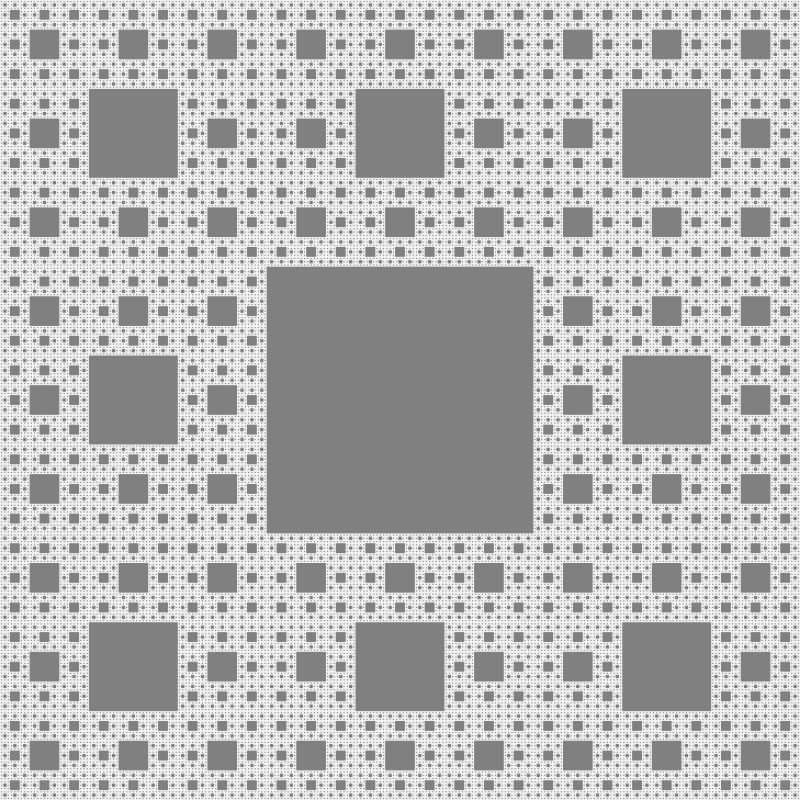
\includegraphics[width=0.35\textwidth]{figure/carpet/carpet.png}
    \caption{Sierpinskiのカーペット}
    \label{pic_carpet}
\end{figure}

Sierpinskiのカーペットは,次の手順\ref{alg_carpet_split}-\ref{alg_carpet_recursion}を繰り返し実行することによって得られます.
\begin{enumerate}
    \enumproc
    \item 与えられた正方形を$3 \times 3$の小正方形に分割する.
        \label{alg_carpet_split}
    \item 分割してできた9個の小正方形のうち,中心にあるものを取り除く.
        \label{alg_carpet_remove}
    \item 残りの8個の小正方形を手順\ref{alg_carpet_split}の正方形とみる.
        \label{alg_carpet_recursion}
\end{enumerate}
%
\begin{figure}[H]
    \centering
    \begin{subfigure}{0.325\textwidth}
        \centering
        
\includegraphics[width=0.7\textwidth]{figure/carpet/carpet_1_split.png}
        \caption{正方形を$3 \times 3$に分割する.}
    \end{subfigure}
    %
    \begin{subfigure}{0.325\textwidth}
        \centering
        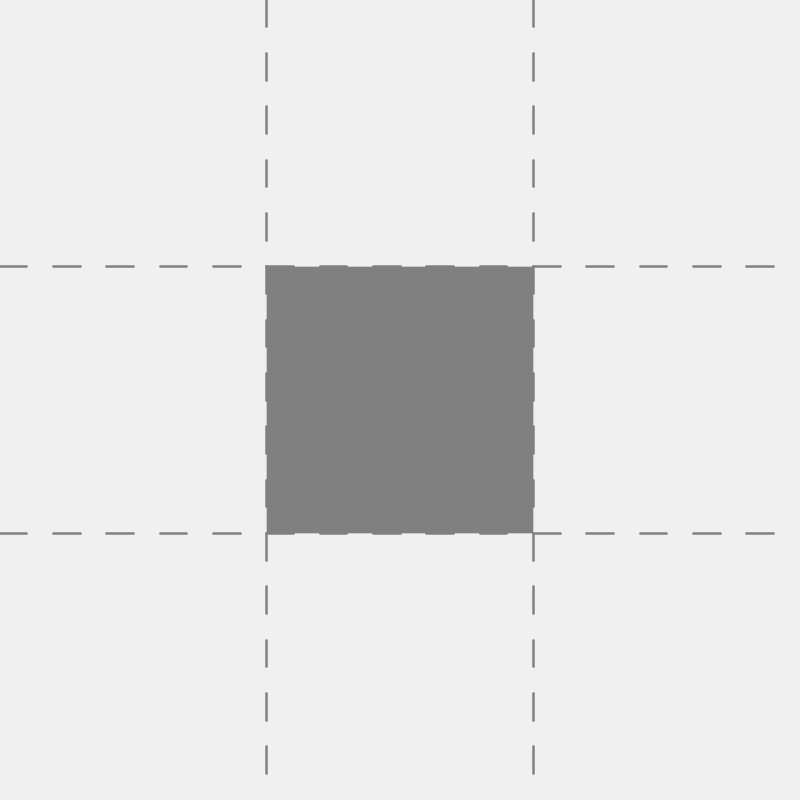
\includegraphics[width=0.7\textwidth]{figure/carpet/carpet_1_fill.png}
        \caption{中心の正方形を取り除く.}
    \end{subfigure}
    %
    \begin{subfigure}{0.325\textwidth}
        \centering
        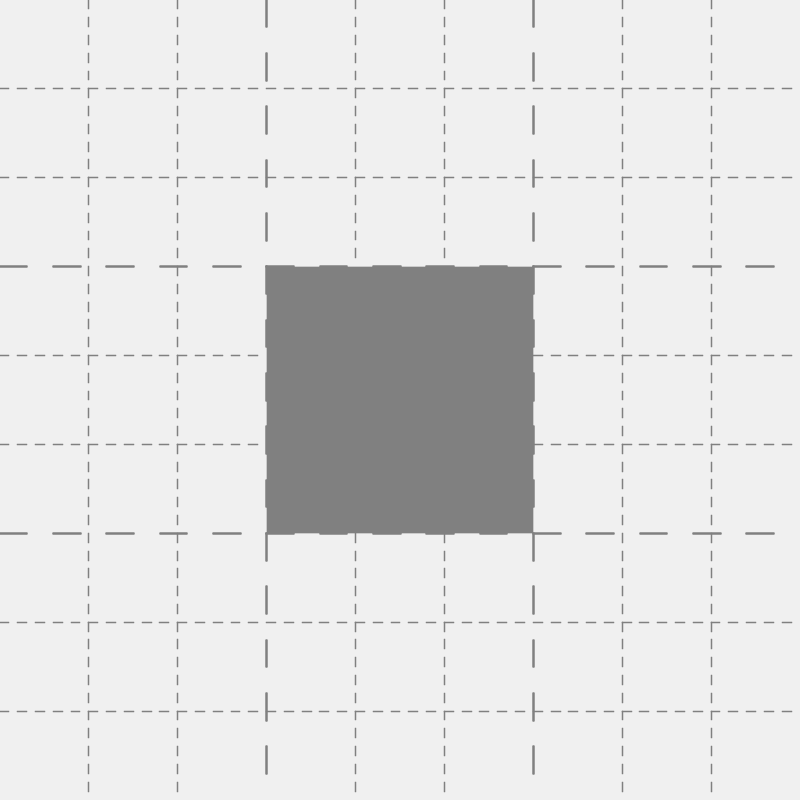
\includegraphics[width=0.7\textwidth]{figure/carpet/carpet_2_split.png}
        \caption{残った正方形を$3 \times 3$に分割する.}
    \end{subfigure}
    %
    \begin{subfigure}{0.325\textwidth}
        \centering
        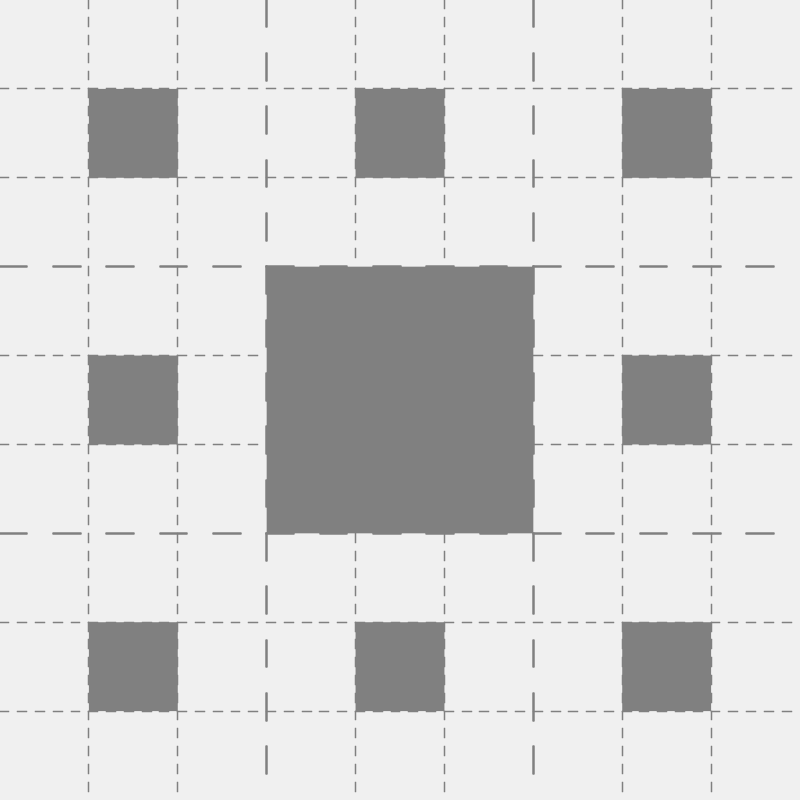
\includegraphics[width=0.7\textwidth]{figure/carpet/carpet_2_fill.png}
        \caption{各正方形の中心を取り除く.}
    \end{subfigure}
    %
    \begin{subfigure}{0.325\textwidth}
        \centering
        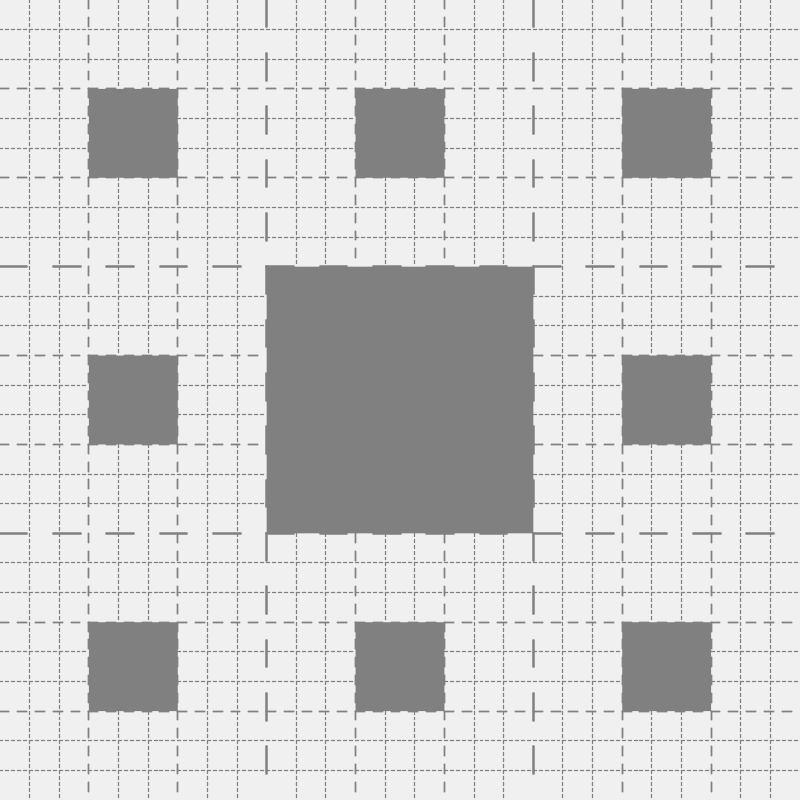
\includegraphics[width=0.7\textwidth]{figure/carpet/carpet_3_split.png}
        \caption{残った正方形を$3 \times 3$に分割する.}
    \end{subfigure}
    %
    \begin{subfigure}{0.325\textwidth}
        \centering
        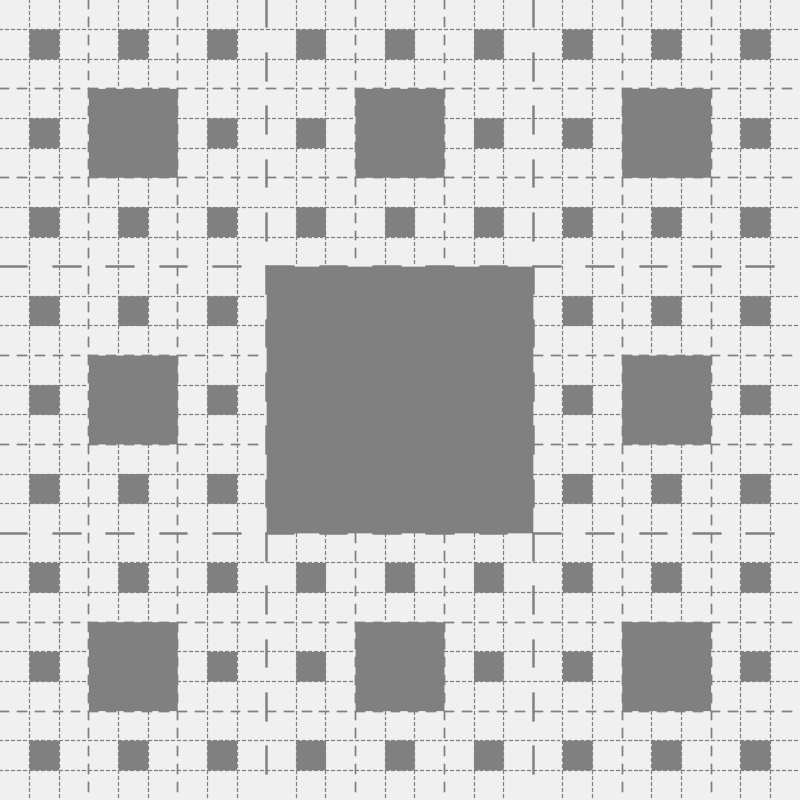
\includegraphics[width=0.7\textwidth]{figure/carpet/carpet_3_fill.png}
        \caption{各正方形の中心を取り除く.}
    \end{subfigure}
    %
    \caption{Sierpinskiのカーペットを描く過程}
    \label{fig_process_carpet}
\end{figure}
%
この操作を再帰関数として記述するとソースコード\ref{code_carpet}のようになります
\footnote{
    p5.jsでは原点が画面左上で$y$軸が下向き正として取られていることに注意してください.
}.
手順\ref{alg_carpet_remove}の正方形の中心を取り除く操作が,正方形を描く関数\verb|square|(8行目)として表されていること,
また,手順\ref{alg_carpet_recursion}の残った8つの正方形をそれぞれひとつの正方形として見る操作が,
関数\verb|carpet|の再帰呼び出し(9-16行目)として表されています.
プログラム全体は\ref{subsec_code_carpet}節に記載しました.
出力は図\ref{pic_carpet}のようになります.
%
\begin{lstlisting}[caption=Sierpinskiのカーペットを描く再帰関数, label=code_carpet]
function carpet(x, y, l, n){  /* 左上座標(x, y),辺lの正方形;再帰の深さn */
    if( n <= 0 ){
        return ;
    }

    let sqlen = l / 3;  // 小正方形の辺の長さ

    square(x+sqlen, y+sqlen, sqlen);  // 中心
    carpet(x        , y        , sqlen, n-1);  // 上左
    carpet(x+sqlen  , y        , sqlen, n-1);  // 上中
    carpet(x+2*sqlen, y        , sqlen, n-1);  // 上右
    carpet(x        , y+sqlen  , sqlen, n-1);  // 中左
    carpet(x+2*sqlen, y+sqlen  , sqlen, n-1);  // 中右
    carpet(x        , y+2*sqlen, sqlen, n-1);  // 下左
    carpet(x+sqlen  , y+2*sqlen, sqlen, n-1);  // 下中
    carpet(x+2*sqlen, y+2*sqlen, sqlen, n-1);  // 下右
}
\end{lstlisting}

Sierpinskiのカーペットは,正方形の一部を取り除くという操作により得られる2次元的な図形
\footnote{
    ここでは,2次元図形である正方形から始めるという意味で,Sierpinskiのカーペットを「2次元的」と表現しています.
}
でした.
これに対し,線分について同様の操作を行うことで得られる1次元的な図形を,Cantor集合(図\ref{pic_cantorset}),
立方体について同様の操作を行うことで得られる3次元的な図形を,Mengerのスポンジ(図\ref{pic_menger_sponge})と呼びます.

\begin{question}
    Sierpinskiのカーペットを描くプログラム(ソースコード\ref{code_carpet_all})を,p5.js Web Editor\cite{p5jseditor}で実行して,
    図\ref{pic_carpet}が出力されることを確認してください.
    また,再帰呼び出しの深さ(ソースコード\ref{code_carpet_all}の11行目,関数\texttt{carpet}の第4引数の値)を変更すると,
    出力される図はどのように変化するか確かめてください.
\end{question}

\begin{question}\label{q_carpet_rec}
    Sierpinskiのカーペットの再帰関数\texttt{carpet}の,
    再帰呼び出し(ソースコード\ref{code_carpet_all}の22-29行目)のいくつかの行を適当にコメントアウトして,
    出力される図がどのように変化するか確かめてください.
\end{question}

\begin{question}
    問\ref{q_carpet_rec}を参考に,Vicsekフラクタル(図\ref{pic_vicfr_x},図\ref{pic_vicfr_c})を描くプログラムを作成してください.
    ヒント:Sierpinskiのカーペットを描くプログラム(ソースコード\ref{code_carpet_all})の,
    中心を塗りつぶす関数\texttt{square}(21行目)を,\texttt{if}文の中(15-16行目の間)へ移動して,
    代わりに中心部分の再帰呼び出し\texttt{carpet}を加える.
\end{question}

\begin{question}
    Cantor集合(図\ref{pic_cantorset})を描くプログラムを作成してください.
\end{question}

\clearpage

%%% -------------------------------------------------------------------------------
\subsection{Sierpinskiのギャスケット}  \label{subsec_gasket}
%%% -------------------------------------------------------------------------------
Sierpinskiのギャスケット
\footnote{
    Sierpinskiの三角形とも呼ばれます.
}
とは,図\ref{pic_gasket}のような,三角形の中心を取り除くという操作を繰り返すことで得られるフラクタル図形です.
\ref{subsec_carpet}節でみたSierpinskiのカーペットの三角形版です.
%
\begin{figure}[H]
    \centering
    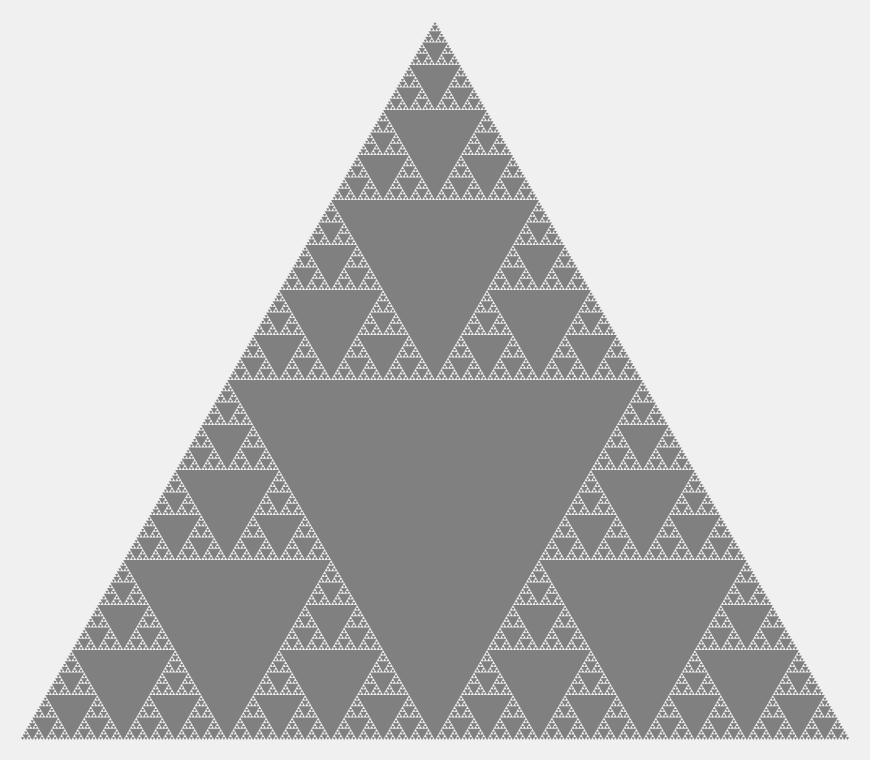
\includegraphics[width=0.4\textwidth]{figure/gasket/gasket.png}
    \caption{Sierpinskiのギャスケット}
    \label{pic_gasket}
\end{figure}

Sierpinskiのギャスケットは,Sierpinskiのカーペットとほぼ同様の手順で得られます.
Sierpinskiのカーペットを得る手順において,正方形を正三角形と読み替えるだけです.
Sierpinskiのギャスケットを描く再帰関数はソースコード\ref{code_gasket}のようになります.
Sierpinskiのカーペットの場合と同様に,正三角形の中心を取り除く操作が,三角形を描く関数\verb|triangle|(14行目)と対応し,
残り3つの正三角形をそれぞれひとつの正三角形として見る操作は,関数\verb|gasket|の再帰呼び出し(15-18行目)と対応します.
プログラム全体は\ref{subsec_code_gasket}節に記載しました.
出力は図\ref{pic_gasket}のようになります.

\begin{lstlisting}[caption=Sierpinskiのギャスケットを描く再帰関数, label=code_gasket]
function gasket(tx, ty, lx, ly, rx, ry, n) {  /* 上頂点(tx, ty),左下頂点(lx, ly),右下頂点(rx, ry)の
                                                 正三角形;再帰の深さn */
    if ( n <= 0 ) {
        return ;
    }

    let lcx = (tx + lx) / 2;  // 上頂点と左下頂点の中点のx座標
    let lcy = (ty + ly) / 2;  // 上頂点と左下頂点の中点のy座標
    let rcx = (tx + rx) / 2;  // 上頂点と右下頂点の中点のx座標
    let rcy = (ty + ry) / 2;  // 上頂点と右下頂点の中点のy座標
    let bcx = (lx + rx) / 2;  // 左下頂点と右下頂点の中点のx座標
    let bcy = (ly + ry) / 2;  // 左下頂点と右下頂点の中点のy座標

    triangle(lcx, lcy, rcx, rcy, bcx, bcy);  // 中心
    gasket(tx , ty , lcx, lcy, rcx, rcy, n-1);  // 上
    gasket(lcx, lcy, lx , ly , bcx, bcy, n-1);  // 左下
    gasket(rcx, rcy, bcx, bcy, rx , ry , n-1);  // 右下
}
\end{lstlisting}

\begin{question}
    正$n$角形を描く関数(ソースコード\ref{code_hexfunc})を参考に,
    Pentaflake(図\ref{pic_penfr}),Hexaflake(図\ref{pic_hexfr})を描くプログラムを作成してください.
    ヒント:再帰の深さが$n$のときの$\{5\mid6\}$角形と,$n-1$のときの$\{5\mid6\}$角形の大きさの比率を考える.
\end{question}

\clearpage

\begin{lstlisting}[caption=正六角形を描く関数, label=code_hexfunc]
function polygon(x, y, l, n) {  /* 中心(x, y)から各頂点までの長さがlの正n角形 */
    beginShape();
    for ( let t = 0; t < TWO_PI; t += TWO_PI/n ) {
        vertex(x+l*cos(t), y+l*sin(t));
    }
    endShape(CLOSE);
}
\end{lstlisting}

%%% -------------------------------------------------------------------------------
\subsection{高木曲線}  \label{subsec_takagi_curve}
%%% -------------------------------------------------------------------------------
高木曲線
\footnote{
    日本の数学者高木貞治(1875-1960)に因みます.
    特徴的な形からブラマンジェ曲線とも呼ばれます.
}
とは,図\ref{pic_takagi_curve}のような,三角波の足し合わせによって得られるフラクタル図形です.
%
\begin{figure}[H]
    \centering
    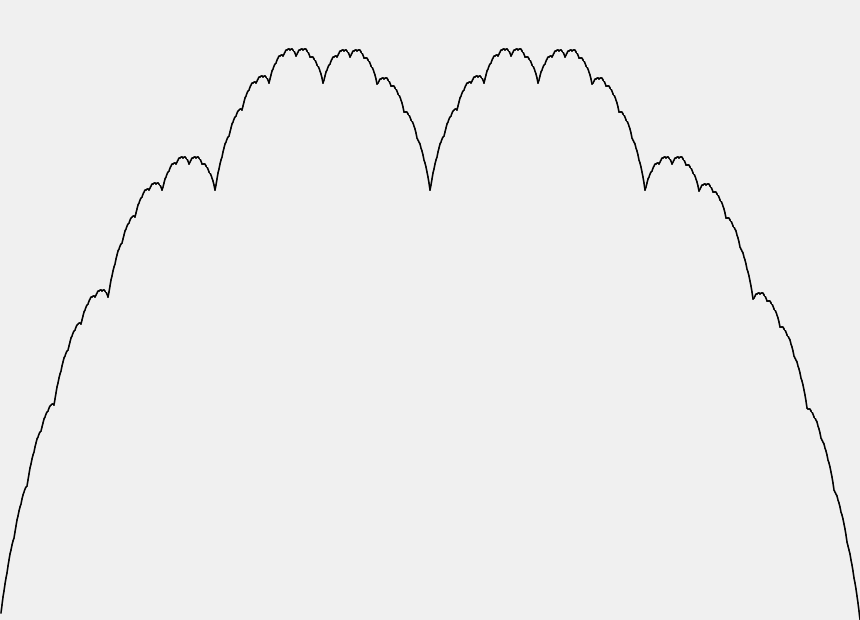
\includegraphics[width=0.4\textwidth]{figure/takagi/takagi_curve.png}
    \caption{高木曲線}
    \label{pic_takagi_curve}
\end{figure}

高木曲線は,次の手順\ref{alg_takagi_tri}-\ref{alg_takagi_recursion}を繰り返し実行することによって得られます.
\begin{enumerate}
    \enumproc
    \item 与えられた区間の中点を頂点とする三角波を考える.
        \label{alg_takagi_tri}
    \item 手順\ref{alg_takagi_tri}の三角波を,これまでに得た全ての三角波を足し合わせたものに加える。
        \label{alg_takagi_add}
    \item 区間を中心で2分割し,左右の小区間を手順\ref{alg_takagi_tri}の区間とみる.
        \label{alg_takagi_recursion}
\end{enumerate}
%
\begin{figure}[H]
    \centering
    \begin{subfigure}{0.24\textwidth}
        \centering
        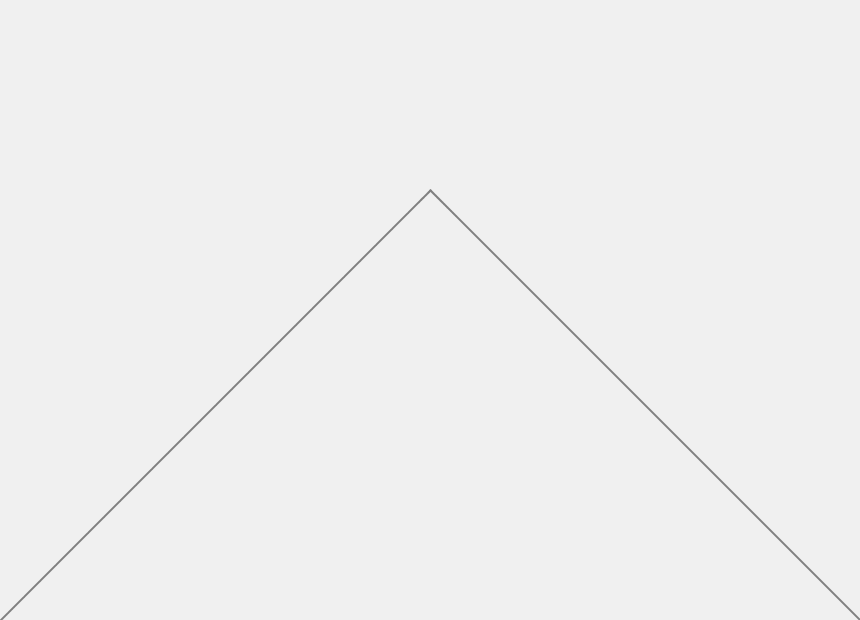
\includegraphics[width=\textwidth]{figure/takagi/takagiwave1.png}
        \caption{区間の中点を頂点とする三角波を考える.}
        \label{fig_proc_takagiwave1}
    \end{subfigure}
    %
    \begin{subfigure}{0.24\textwidth}
        \centering
        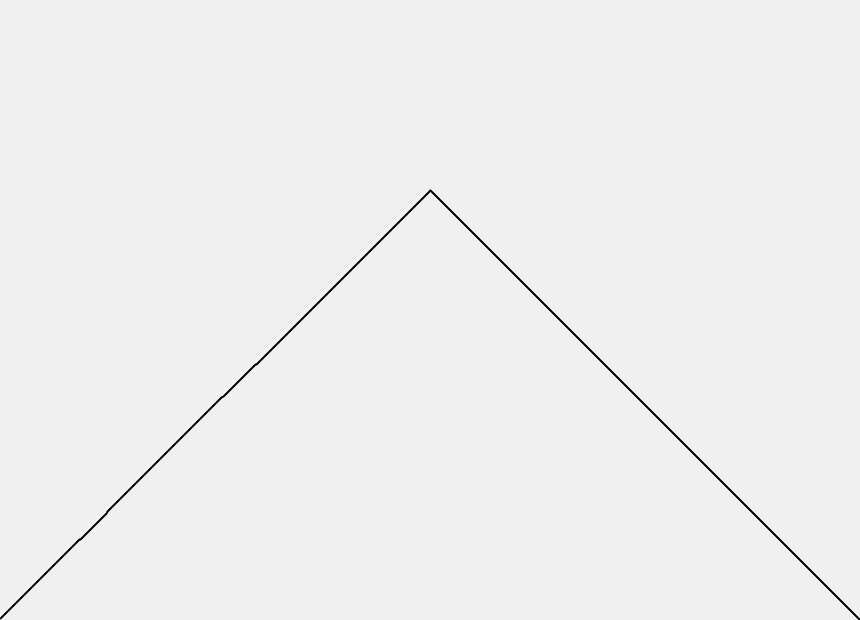
\includegraphics[width=\textwidth]{figure/takagi/takagicurve1.png}
        \caption{(\subref{fig_proc_takagiwave1})の三角波を初期状態(高さ0の波)に足し合わせる.}
        \label{fig_proc_takagicurve1}
    \end{subfigure}
    %
    \begin{subfigure}{0.24\textwidth}
        \centering
        
\includegraphics[width=\textwidth]{figure/takagi/takagiwave2.png}
        \caption{(\subref{fig_proc_takagiwave1})の区間を2等分してそれぞれ三角波を考える.}
        \label{fig_proc_takagiwave2}
    \end{subfigure}
    %
    \begin{subfigure}{0.24\textwidth}
        \centering
        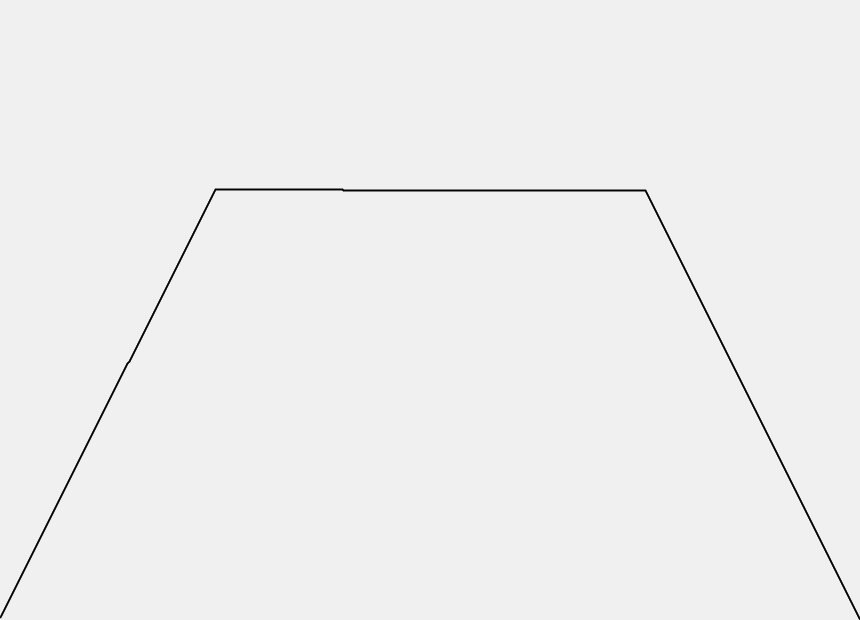
\includegraphics[width=\textwidth]{figure/takagi/takagicurve2.png}
        \caption{(\subref{fig_proc_takagiwave2})の三角波を(\subref{fig_proc_takagicurve1})に足し合わせる.}
        \label{fig_proc_takagicurve2}
    \end{subfigure}
    %
    \begin{subfigure}{0.24\textwidth}
        \centering
        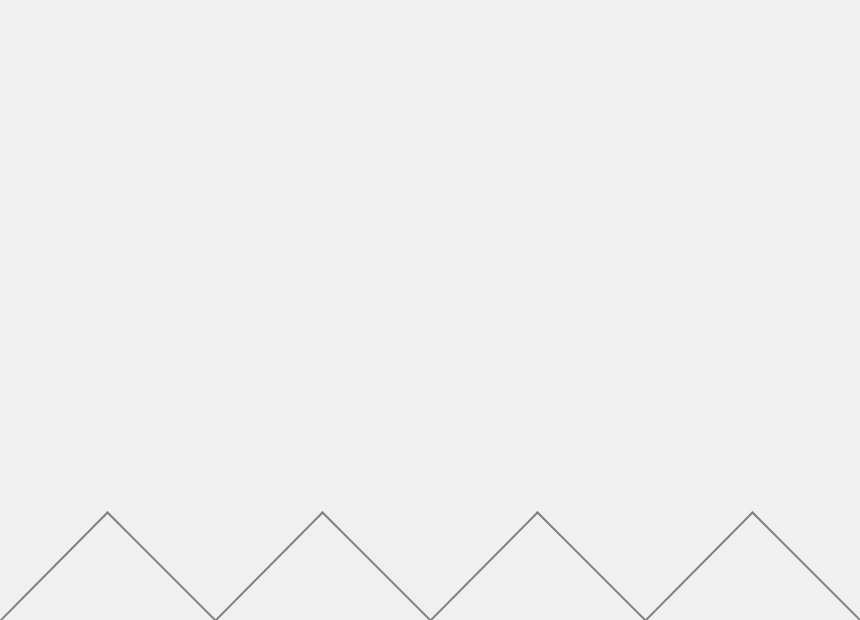
\includegraphics[width=\textwidth]{figure/takagi/takagiwave3.png}
        \caption{(\subref{fig_proc_takagiwave2})の各区間を2等分してそれぞれ三角波を考える.}
        \label{fig_proc_takagiwave3}
    \end{subfigure}
    %
    \begin{subfigure}{0.24\textwidth}
        \centering
        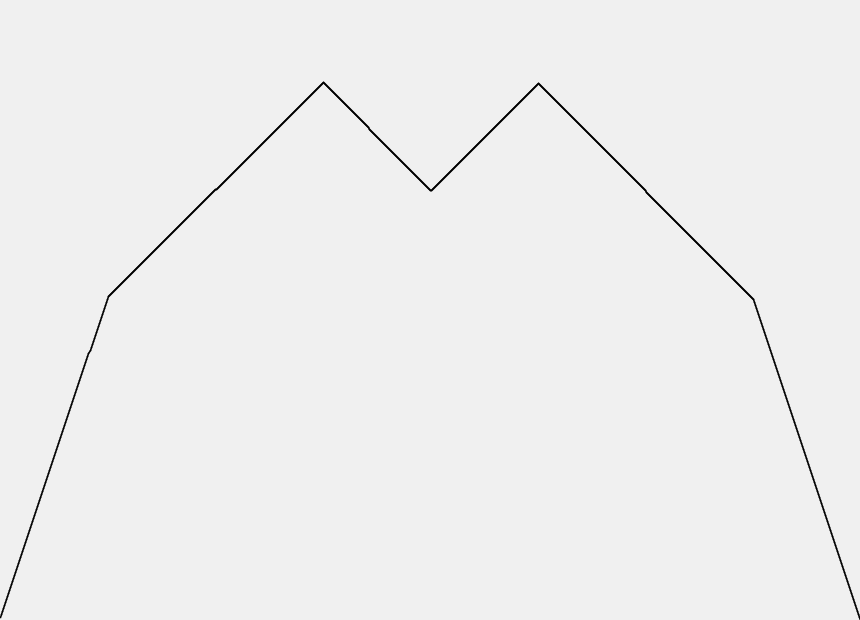
\includegraphics[width=\textwidth]{figure/takagi/takagicurve3.png}
        \caption{(\subref{fig_proc_takagiwave3})の三角波を(\subref{fig_proc_takagicurve2})に足し合わせる.}
        \label{fig_proc_takagicurve3}
    \end{subfigure}
    %
    \begin{subfigure}{0.24\textwidth}
        \centering
        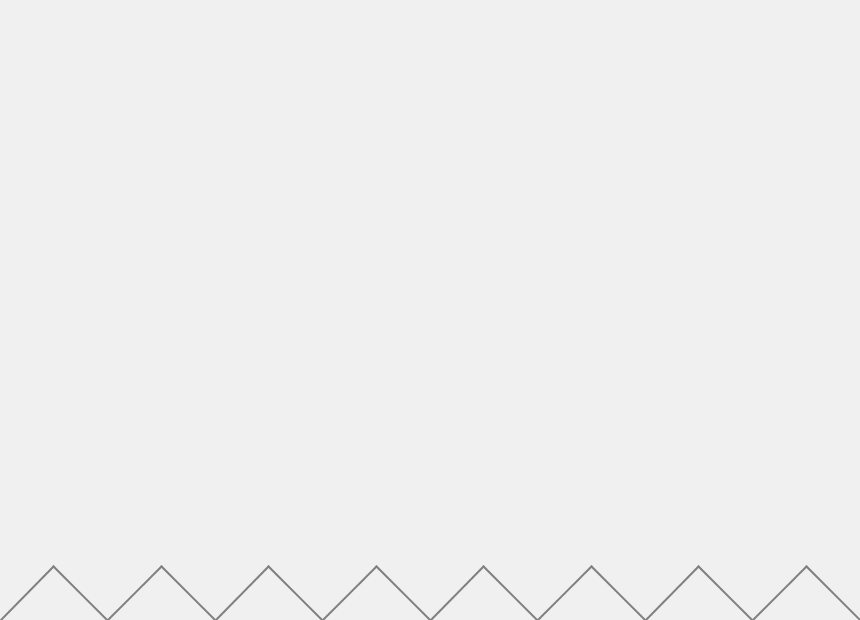
\includegraphics[width=\textwidth]{figure/takagi/takagiwave4.png}
        \caption{(\subref{fig_proc_takagiwave3})の各区間を2等分してそれぞれ三角波を考える.}
        \label{fig_proc_takagiwave4}
    \end{subfigure}
    %
    \begin{subfigure}{0.24\textwidth}
        \centering
        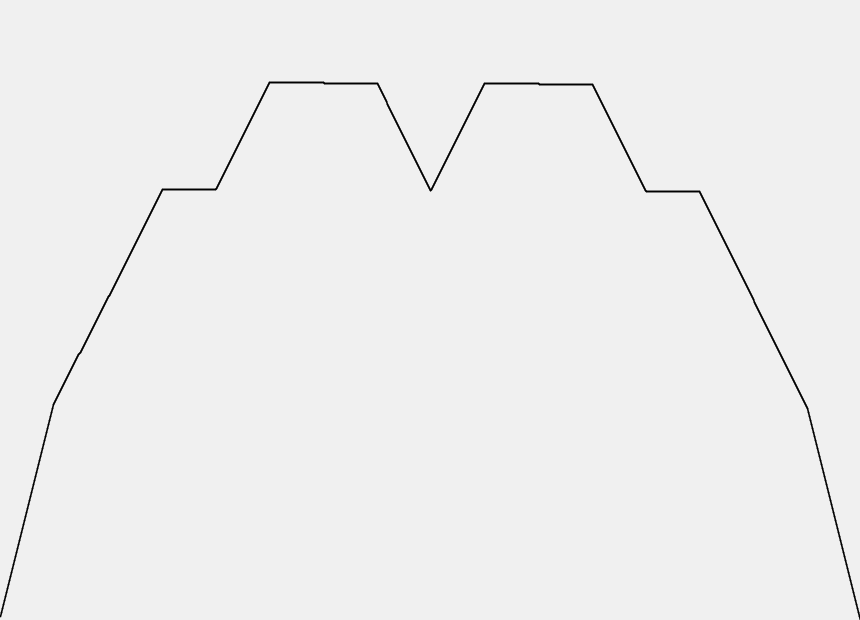
\includegraphics[width=\textwidth]{figure/takagi/takagicurve4.png}
        \caption{(\subref{fig_proc_takagiwave4})の三角波を(\subref{fig_proc_takagicurve3})に足し合わせる.}
        \label{fig_proc_takagicurve4}
    \end{subfigure}
    %
    \caption{高木曲線を描く過程}
    \label{fig_process_takagi_curve}
\end{figure}
%
この操作を再帰関数として記述するとソースコード\ref{code_takagi_curve}のようになります.
\verb|ys|は,これまでに得た全ての三角波を足し合わせた曲線の,位置\verb|x|における高さを保持する配列です.
手順\ref{alg_takagi_tri}-\ref{alg_takagi_add}の三角波の足し合わせが,10-15行目の\verb|for|文の処理と対応し,
手順\ref{alg_takagi_recursion}の左右の小区間をそれぞれひとつの区間として見る操作は,
関数\verb|takagicurve|の再帰呼び出し(16-17行目)と対応します.
%
プログラム全体は\ref{subsec_code_takagi_curve}節に記載しました.
出力は図\ref{pic_takagi_curve}のようになります.
%
\begin{lstlisting}[caption=高木曲線を描く再帰関数, label=code_takagi_curve]
function takagicurve(lx, rx, n) {  /* 区間[lx, rx],再帰の深さn */
    if( n <= 0 ){
        return ;
    }

    let cx = int((lx + rx) / 2);  // 区間の中点
    let y = 0;                    // 三角波の高さ

    // 三角波の足し合わせ(ysは位置xにおける高さを保持する配列)
    for ( let x = lx; x < cx; x++ ) {
        ys[x] += y++;
    }
    for ( let x = cx; x < rx; x++ ) {
        ys[x] += y--;
    }
    takagicurve(lx, cx, n-1);  // 左
    takagicurve(cx, rx, n-1);  // 右
}
\end{lstlisting}

高木曲線は,連続且つ至る所で微分不可能であるという性質を持ちます.
\begin{comment}
高木曲線は,連続且つ至る所で微分不可能であるという性質を持ち,次のような関数$T(x)$として表されます.
\begin{align*}
    T(x) = \sum_{n=0}^{\infty} \frac{\gamma(2^n x)}{2^n}
\end{align*}
ここで$\gamma(x)$は次のように定められる三角波関数です.
\begin{align*}
    \gamma(x) = \min_{m \in \mathbb{Z}} |x - m|
\end{align*}
\end{comment}

\begin{question}
    高木曲線の他にも,連続且つ至る所で微分不可能という性質を持つ関数として,Weierstrass関数があります.
    Weierstrass関数について調べてみてください。
\end{question}

%%% -------------------------------------------------------------------------------
\subsection{Koch曲線}  \label{subsec_koch_curve}
%%% -------------------------------------------------------------------------------
Koch曲線
\footnote{
    スウェーデンの数学者Helge von Koch(1870-1924)に因みます.
}
とは,図\ref{pic_koch_curve}のような,線分を3分割し,その中央の部分を山形にするという操作を繰り返すことで得られるフラクタル図形です.
%
\begin{figure}[H]
    \centering
    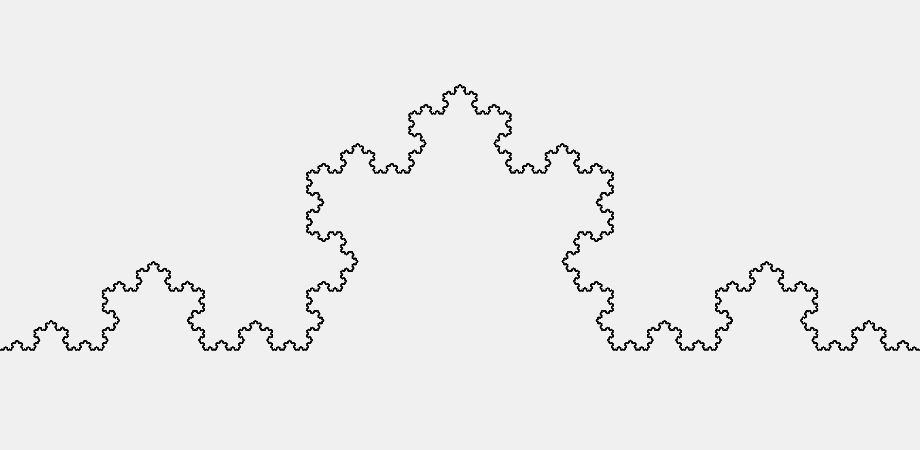
\includegraphics[width=0.55\textwidth]{figure/koch/koch_curve.png}
    \caption{Koch曲線}
    \label{pic_koch_curve}
\end{figure}

Koch曲線は,次の手順\ref{alg_koch_split}-\ref{alg_koch_recursion}を繰り返し実行することによって得られます.
\begin{enumerate}
    \enumproc
    \item 与えられた線分を3つの小線分に3等分する.
        \label{alg_koch_split}
    \item 中央の小線分を,小線分を1辺とするような正三角形の残りの2辺と置き換える.
        \label{alg_koch_replace}
    \item 4つの小線分を手順\ref{alg_koch_split}の線分とみる.
        \label{alg_koch_recursion}
\end{enumerate}
%
\begin{figure}[H]
    \centering
    \begin{subfigure}{0.325\textwidth}
        \centering
        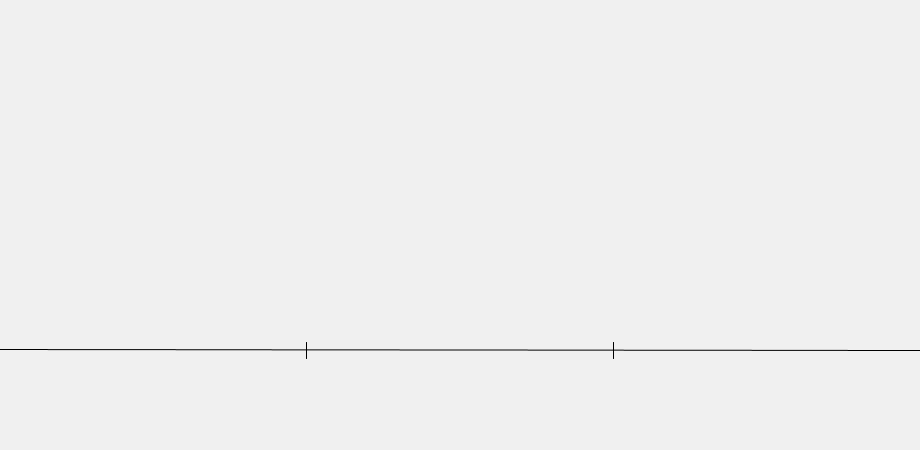
\includegraphics[width=\textwidth]{figure/koch/koch_curve0_split.png}
        \caption{線分を3等分する.}
        \label{fig_proc_kochcurve0_split}
    \end{subfigure}
    %
    \begin{subfigure}{0.325\textwidth}
        \centering
        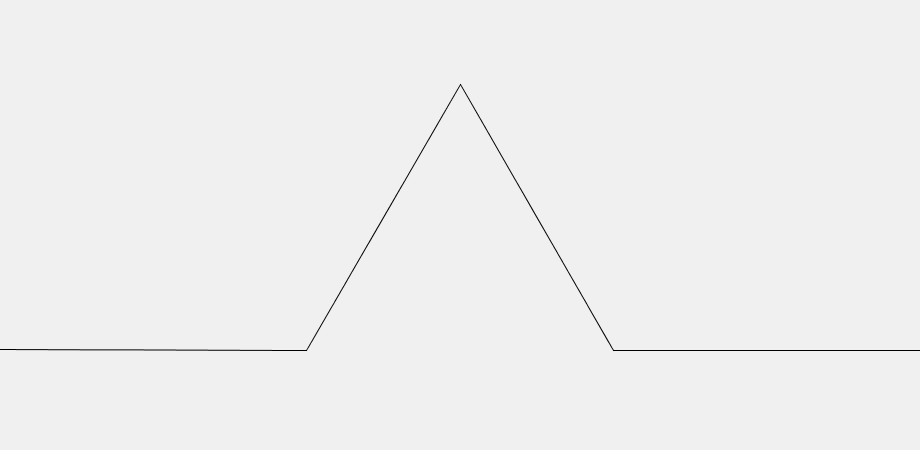
\includegraphics[width=\textwidth]{figure/koch/koch_curve1.png}
        \caption{中央を正三角形の2辺で置き換える.}
        \label{fig_proc_kochcurve1}
    \end{subfigure}
    %
    \begin{subfigure}{0.325\textwidth}
        \centering
        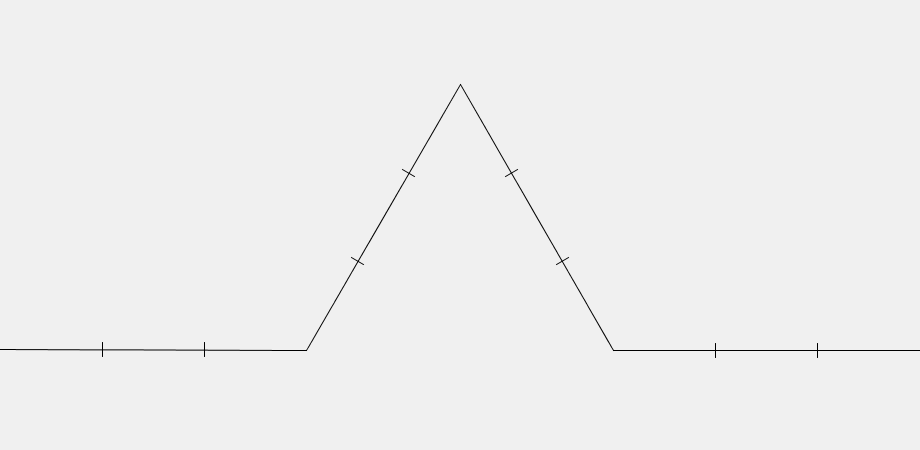
\includegraphics[width=\textwidth]{figure/koch/koch_curve1_split.png}
        \caption{4辺をそれぞれ3等分する.}
        \label{fig_proc_kochcurve1_split}
    \end{subfigure}
    %
    \begin{subfigure}{0.325\textwidth}
        \centering
        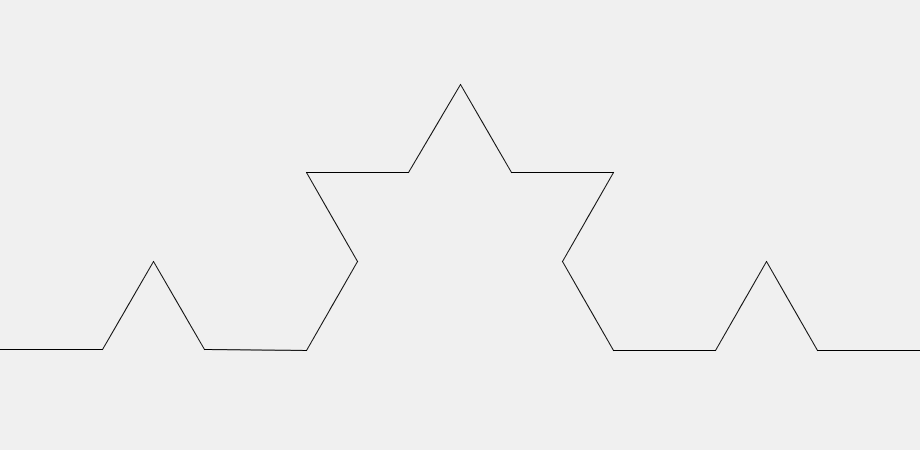
\includegraphics[width=\textwidth]{figure/koch/koch_curve2.png}
        \caption{中央を正三角形の2辺で置き換える.}
        \label{fig_proc_kochcurve2}
    \end{subfigure}
    %
    \begin{subfigure}{0.325\textwidth}
        \centering
        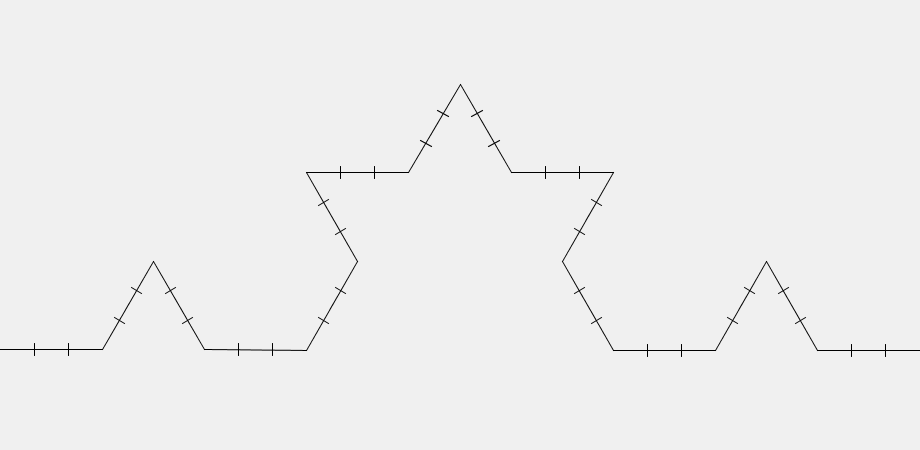
\includegraphics[width=\textwidth]{figure/koch/koch_curve2_split.png}
        \caption{各辺をそれぞれ3等分する.}
        \label{fig_proc_kochcurve2_split}
    \end{subfigure}
    %
    \begin{subfigure}{0.325\textwidth}
        \centering
        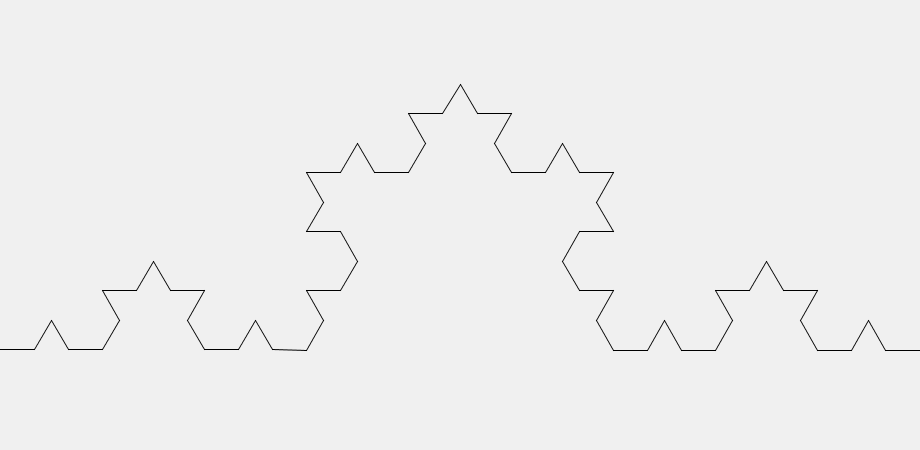
\includegraphics[width=\textwidth]{figure/koch/koch_curve3.png}
        \caption{中央を正三角形の2辺で置き換える.}
        \label{fig_proc_kochcurve3}
    \end{subfigure}
    %
    \caption{Koch曲線を描く過程}
    \label{fig_process_koch_curve}
\end{figure}
%
この操作を再帰関数として記述するとソースコード\ref{code_koch_curve}のようになります.
手順\ref{alg_koch_recursion}の4つの線分をそれぞれひとつの線分として見る操作が,関数\verb|kochcurve|の再帰呼び出し(12-15行目)と対応します.
2-3つ目の再帰呼び出し(13-14行目)が,手順\ref{alg_koch_replace}の正三角形の2辺と対応していることに注意してください.
プログラム全体は\ref{subsec_code_koch_curve}節に記載しました.
出力は図\ref{pic_koch_curve}のようになります.
%
\begin{lstlisting}[caption=Koch曲線を描く再帰関数, label=code_koch_curve]
function kochcurve(lx, ly, rx, ry, n) {  /* 左端(lx, ly),右端(rx, ry)の線分;再帰の深さn */
    if ( n <= 0 ) {
        line(lx, ly, rx, ry);
        return ;
    }

    let dx = (rx - lx) / 3;  // 小線分x成分
    let dy = (ry - ly) / 3;  // 小線分y成分
    let cx = (lx + rx) / 2;  // 線分の中点のx座標
    let cy = (ly + ry) / 2;  // 線分の中点のy座標

    kochcurve(lx             , ly             , lx+dx          , ly+dy          , n-1);  // 左
    kochcurve(lx+dx          , ly+dy          , cx-sqrt(3)/2*dy, cy+sqrt(3)/2*dx, n-1);  // 中左
    kochcurve(cx-sqrt(3)/2*dy, cy+sqrt(3)/2*dx, rx-dx          , ry-dy          , n-1);  // 中右
    kochcurve(rx-dx          , ry-dy          , rx             , ry             , n-1);  // 右
}
\end{lstlisting}

Koch曲線も高木曲線と同様,連続且つ至る所で微分不可能であるという性質を持ちます.
また,図\ref{pic_koch_snowflake}の様に,3つのKoch曲線を星形のように繋げた図形をKoch雪片といいます.

\begin{question}
    Koch曲線の長さは無限大であることを示してください.
\end{question}

\begin{question}
    最初の正三角形の1辺の長さを$l$として,Koch雪片の面積を求めてください.
\end{question}

%%% -------------------------------------------------------------------------------
\subsection{再帰的定義}  \label{subsec_recursion}
%%% -------------------------------------------------------------------------------
この章では,再帰関数によってフラクタル図形を描いてきました.
再帰関数(再帰的定義)は,数学やプログラミングにおいて,フラクタル以外の場面でも頻繁に登場します.
身近な例では,総和演算子$\Sigma$は,次のように再帰的に定められます.
%
\begin{align*}
    \sum_{i=0}^{n} x_i \coloneqq
        \begin{dcases}
            x_0 & (n = 0) \\
            x_n + \sum_{i=0}^{n-1} x_i & (n \geq 1)
        \end{dcases}
\end{align*}
%
これをp5.jsの再帰関数として書くと,ソースコード\ref{code_recursive_sum}のようになります.
プログラム全体は\ref{subsec_code_recursive_sum}節に記載しました.
%
\begin{lstlisting}[caption=総和を計算する再帰関数, label=code_recursive_sum]
/* 配列xsの要素の総和を求める関数 */
function recursive_sum(xs, n){  /* 配列xs=[x0,x1,...,xn];再帰の深さn */
    if( n == 0 ){
        return xs[n];
    }
    return xs[n] + recursive_sum(xs, n-1);
}
\end{lstlisting}

\begin{question}
    総乗演算子$\Pi$,階乗演算子$!$も再帰的に定義されます.
    配列\verb|xs|の総和を計算する再帰関数(ソースコード\ref{code_recursive_sum})を参考に,
    配列\verb|xs|の総乗を計算する再帰関数\verb|recursive_prod(xs, n)|,
    $n$の階乗を計算する再帰関数\verb|recursive_factorial(n)|を作成してください.
\end{question}

\begin{question}
    次のように定義される数列${a_n}$をFibonacci数列と言います.
    \begin{align*}
        a_n \coloneqq
            \begin{cases}
                1 & (n = 0, 1) \\
                a_{n-1} + a_{n-2} & (n \geq 2)
            \end{cases}
    \end{align*}
    Fibonacci数列の第$n$項を計算する再帰関数\verb|recursive_fib(n)|を作成してください.
\end{question}

\begin{question}
    $n \in \mathbb{N}, \ 0 \leq k \leq n$に対して,二項係数$\dbinom{n}{k}$
    \footnote{
        ${}_{n}\mathrm{C}_{k}$と表記される場合もあります.
    }
    は次のように定義されます.
    \begin{align*}
        \binom{n}{k} \coloneqq
            \begin{dcases}
                \quad 1 & (k=0, n) \\
                \binom{n-1}{k} + \binom{n-1}{k-1} & (k \neq 0, n)
            \end{dcases}
    \end{align*}
    二項係数$\dbinom{n}{k}$を計算する再帰関数\verb|recursive_binom(n, k)|を作成してください.
\end{question}

\begin{question}
    図\ref{fig_pascal_tri}のように,二項係数をピラミッド状に並べたものを,Pascalの三角形
    \footnote{
        Pascalの三角形や二項係数について,詳しくは\cite{eular}などを参照して下さい.
    }
    と言います.
    Pascalの三角形を,偶数・奇数で色を塗り分けると,どのような模様が現れるでしょうか.
    %
    \begin{figure}[H]
        \centering
        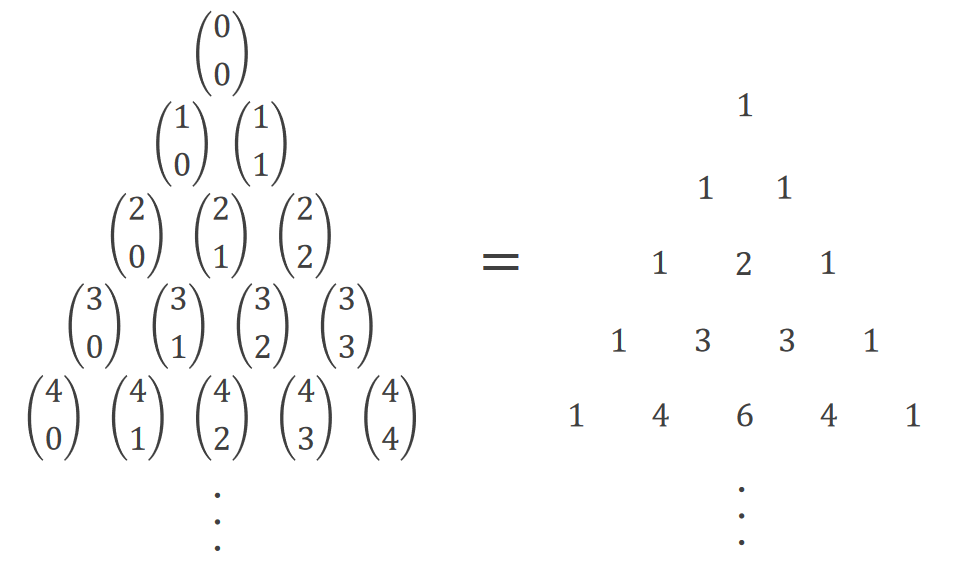
\includegraphics[width=0.55\textwidth]{figure/others/pascal_tri.png}
        \caption{Pascalの三角形}
        \label{fig_pascal_tri}
    \end{figure}
\end{question}

\clearpage


%%% ===============================================================================
\section{セルオートマトン}  \label{sec_cellular_automaton}
%%% ===============================================================================
セルオートマトンとは,空間内に固定配置された多数のセルが,局所的に作用し合うことで状態を変化させていくようなシステムのことをいいます.
セルオートマトンの例として,John Horton Conway(1937-2020)が考案したライフゲームが有名です.
%
\begin{figure}[H]
    \centering
    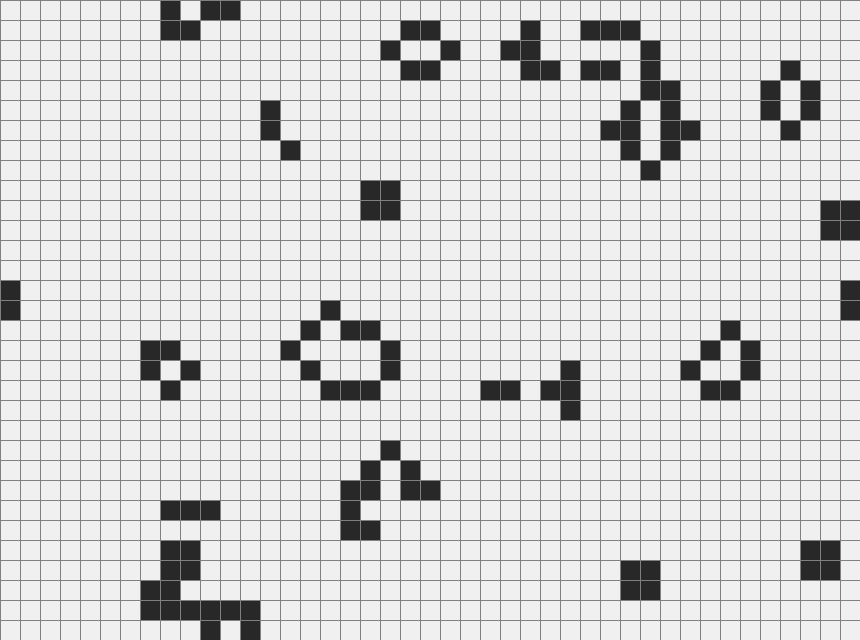
\includegraphics[scale=0.25]{figure/eca/lifegame.png}
    \caption{
        ライフゲーム:
        黒いマスが生きたセル,白いマスが死んだセルを表す.
        周囲のセルの状態によってセルの生存・死滅が決定する.
        周期的に振動するものや移動するものなど様々なパターンが現れる.
    }
    \label{pic_lifegame}
\end{figure}

セルが直線状(1次元上)に配置されたセルオートマトンを,1次元セルオートマトンと呼びます
\footnote{
    セルが平面上に配置されるライフゲームは2次元セルオートマトンです.
    図\ref{pic_lifegame}は,2次元のセルオートマトンの1時刻の状態を表した図です.
    1次元セルオートマトンの1時刻の状態を上から順に並べて遷移を可視化した図\ref{pic_eca}との違いに注意してください.
}.
また,1次元のセルオートマトンでセルの状態が2値$\{0, 1\}$のいずれかをとり,
セルの次の状態が自身と隣接する2つのセルの状態によって決定されるものを,基本セルオートマトンと呼びます
\footnote{
    特徴を列挙して,1次元2状態3近傍セルオートマトンと呼ぶこともあります.
}.
この章では,基本セルオートマトンについて見ていきます.

%%% -------------------------------------------------------------------------------
\subsection{状態遷移とWolframコード}  \label{subsec_trans_wcode}
%%% -------------------------------------------------------------------------------
基本セルオートマトンでは,あるセルの時刻$t+1$の状態は,そのセルと隣接する2つ(左隣・右隣)のセルの時刻$t$の状態によって決定されます.
%
\begin{figure}[H]
    \centering
    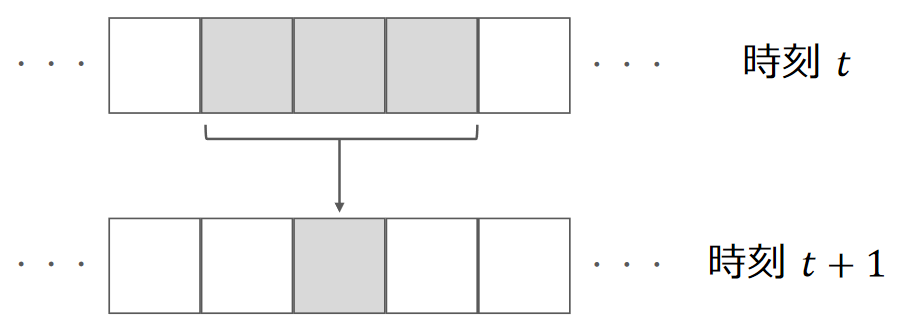
\includegraphics[scale=0.2]{figure/eca/eca_trans.png}
    \caption{
        基本セルオートマトンの遷移:
        時刻$t+1$のセル(下列灰色のセル)の状態は,
        時刻$t$におけるそのセル自身の状態と隣接する2つのセル(上列灰色のセル)の状態によって決定される.
    }
    \label{pic_eca_trans}
\end{figure}

3つのセルの現在の状態から,セルの次の状態を決定するための遷移規則について考えましょう.
今,セルの状態が2通りの基本セルオートマトンを考えているので,遷移前の3つのセルの状態の組み合わせは全部で$2^3$通り存在します.
また,遷移後のセルの状態は,$\{0,1\}$の2通りです.
遷移前の状態が8通り,遷移後の状態が2通りあるので,遷移の規則は全部で$2^8$通り存在します.

この256通りの遷移規則を区別するため,それぞれの遷移規則に番号を割り当てます.
遷移後のセルの状態を順に並べ,その数字列を2進数として見たときの数を,それぞれの規則に割り当てます.
表\ref{tab_transrule_150}の遷移規則を例として説明します.
%
\begin{table}[H]
    \caption{遷移規則(ルール150)}
    \label{tab_transrule_150}
    \centering
    \begin{tabular}{|c||c|c|c|c|c|c|c|c|} \hline
        自身及び隣接するセルの状態 & 111 & 110 & 101 & 100 & 011 & 010 & 001 & 000 \\ \hline
        遷移後のセルの状態      &  1  &  0  &  0  &  1  &  0  &  1  &  1  &  0  \\ \hline
    \end{tabular}
\end{table}
%
\noindent
この遷移規則における遷移後の状態(表\ref{tab_transrule_150}下行)を,左から順に並べると$(1, 0, 0, 1, 0, 1, 1, 0)$となっています.
これを2進数とみると$10010110_{(2)} = 1\times 2^7 + 1\times 2^4 + 1\times 2^2 + 1\times 2^1 = 150$となるので,表1の遷移規則をルール150と呼びます.
この他の遷移規則についても同様に番号を割り当てます.
このようにして割り当てられた遷移規則の番号をWolframコードと呼びます
\footnote{
    この名前はStephen Wolframに因みます.
    Stephen Wolframはセルオートマトンの解析の他に,MathmaticaやWolfram Alpha\cite{wolalp}の開発でも有名です.
}.

\begin{example}
    \label{ex_transrule}
    表\ref{tab_transrule_90}のような遷移規則は,ルール90と呼ばれます.
    %%%
    \begin{table}[H]
        \caption{遷移規則(ルール90)}
        \label{tab_transrule_90}
        \centering
        \begin{tabular}{|c||c|c|c|c|c|c|c|c|} \hline
            自身及び隣接するセルの状態 & 111 & 110 & 101 & 100 & 011 & 010 & 001 & 000 \\ \hline
            遷移後のセルの状態      &  0   &  1  &  0  &  1  &  1  &  0  &  1  &  0 \\ \hline
        \end{tabular}
    \end{table}
\end{example}

\begin{example}
    \label{ex_update_gen}
    現在のセルの状態が\verb|"01011100"|であるような基本セルオートマトンの状態遷移を考えます.
    遷移規則はルール150として,両端は繋がっているとします.
    %%%
    \begin{table}[H]
        \caption{ルール150に従う遷移計算の例}
        \label{tab_ex_update_gen}
        \centering
        \begin{tabular}{|c||c|c|c|c|c|c|c|c|} \hline
            現在のセルの状態 & 0 & 1 & 0 & 1 & 1 & 1 & 0 & 0 \\ \hline
            自身及び隣接するセルの状態 & 001 & 010 & 101 & 011 & 111 & 110 & 100 & 000 \\ \hline
            遷移後のセルの状態 & 1 & 1 & 0 & 0 & 1 & 0 & 1 & 0 \\ \hline
        \end{tabular}
    \end{table}
    %%%
    各セルの状態遷移は表\ref{tab_ex_update_gen}のように計算されます.
    遷移後のセルの状態は\verb|"11001010"|となります.
\end{example}

最後に,遷移規則をプログラムで表すことを考えます.
ここではルール150に従った状態遷移,つまり表\ref{tab_transrule_150}を関数として実装します.
関数はソースコード\ref{code_update}のように書けます.

\begin{lstlisting}[caption=ルール150に基づく遷移を計算する関数, label=code_update]
function updateState(l, t, r) {  /* ルール150に従い,3つのセルの状態(l, t, r)から次の状態を計算 */
    let binnum = 4*l + 2*t + 1*r;              // 3つのセルの状態の列を2進数とみたときの数 [0,1,..,7]
    const rule150 = [0, 1, 1, 0, 1, 0, 0, 1];  // ルール150における遷移後の状態を持つ配列
    return rule150[binnum];
}
\end{lstlisting}

基本セルオートマトンでは,状態は$\{0,1\}$の2通りなので,遷移前の3つのセルの状態の並びを2進数として見ると,
0から7の自然数となります(2行目の変数\verb|binom|).
また,遷移後の状態を,配列\verb|rule150|の\verb|binom|番目に配置しています(3行目)
\footnote{
    配列は0番目から順に格納されるので,表\ref{tab_transrule_150}下行とは逆順で数が格納されることに注意してください.
}.
%
例えば,遷移前の状態が\verb|(l,t,r)=(1,0,1)|の場合,\verb|binom=5|となり,
配列\verb|rule150|の\verb|binom=5|番目の値を参照すれば,遷移後の状態\verb|rule150[5]=0|が得られます.

%%% -------------------------------------------------------------------------------
\subsection{実装}  \label{subsec_implementation}
%%% -------------------------------------------------------------------------------
ここからは,いくつかの関数を実装して,基本セルオートマトンのプログラムを完成させます.
以降の説明において,$n$回状態遷移を行ったセルを第$n$世代のセルと呼ぶことにします.

%%% ...............................................................................
\subsubsection{大域変数}  \label{subsubsec_global_var}
%%% ...............................................................................
定義する大域変数をソースコード\ref{code_globalvar}に示します.
セルの描画サイズを\verb|SQSIZE|として与えています.
これはセルの描画の他に,セルの個数(配列\verb|cells|の要素数)・世代数の決定で使われることになります.
また,\verb|cells|はセルの状態を保持する配列です.
セルの世代更新はこの配列が持つ値の更新として行います.
%
\begin{lstlisting}[caption=大域変数, label=code_globalvar]
const SQSIZE = 8.0;  // セルの描画サイズ(定数)
let cells;           // セルの状態を保持する配列
\end{lstlisting}

%%% ...............................................................................
\subsubsection{セルの初期化}  \label{subsubsec_cell_init}
%%% ...............................................................................
セルの初期化を行う関数をソースコード\ref{code_cellinit}に示します.
この関数では,セルの状態を保持する配列\verb|cells|に初期状態(第0世代の状態)を与えます.
初期状態は,中央のセルのみを1,それ以外は0としています.
また,セルの個数は,描画時に画面に入る最大の数としています
\footnote{
    \label{fnote_display_window}
    p5.jsにおいて,変数\texttt{width}はウィンドウ(図形が表示される場所)の幅を保持するシステム変数です.
    また,対になる変数\texttt{height}はウィンドウの高さを保持します.
    いま,セルの描画サイズは\texttt{SQSIZE}で与えられているので,ウィンドウ(幅)に入る最大のセル個数は\texttt{int(width/SQSIZE)}で得られます.
}.
%
\begin{lstlisting}[caption=セルの初期化関数, label=code_cellinit]
function initCells() {
    const cellsLength = int(width / SQSIZE);  // セルの個数(配列cellsの要素数)
    cells = [];
    for ( let i = 0; i < cellsLength; i++ ) {
        cells[i] = ( i == int(cellsLength/2) )? 1 : 0;  // 中央のセルのみ1,それ以外は0で初期化
    }
}
\end{lstlisting}

%%% ...............................................................................
\subsubsection{世代更新}  \label{subsubsec_gen_update}
%%% ...............................................................................
世代更新(状態遷移)を行う関数をソースコード\ref{code_cellupdate}に示します.
5-7行目で遷移前のセルの状態を配列\verb|cpcells|に保存(コピー)した後,
9-13行目で配列\verb|cpcells|の値と関数\verb|updateCells|により,セルの状態(配列\verb|cells|の値)を更新しています
\footnote{
    この関数では,遷移前の状態を保持しておかないと世代更新は正しく行われません.
    状態遷移は添字が小さいほうから順に行われていくので,
    例えば,\texttt{i = 1}の場合,\texttt{cells[1] = updateState(cells[0], cells[1], cells[2]);}としてしまうと,
    \texttt{cells[0]}は遷移後の状態を持ち,\texttt{cells[1]}の遷移が正しく行われなくなります.
}.
またこのとき,両端(\verb|cell.length-1|番目のセルと\verb|0|番目のセル)は繋がっているとして,遷移を行います
\footnote{
    添字の剰余計算を利用します.
    \texttt{i = 0}の場合に添字が負数になることを防ぐために,左隣のセルの添字のみ\texttt{cells.length}を加算してから計算しています.
}.
%
\begin{lstlisting}[caption=世代更新関数, label=code_cellupdate]
function updateCells() {
    let cpcells = [];  // 遷移前のセルの状態を保持する配列

    /* 遷移前のセルの状態の保存 */
    for ( let i = 0; i < cells.length; i++ ) {
        cpcells[i] = cells[i];
    }
    /* 世代更新 (全セルの状態遷移) */
    for ( let i = 0; i < cells.length; i++ ) {
        cells[i] = updateState(cpcells[(i-1+cells.length)%cells.length],
                               cpcells[i],
                               cpcells[(i+1)%cells.length]);
    }
}
\end{lstlisting}

%%% ...............................................................................
\subsubsection{セルの描画}  \label{subsubsec_cell_draw}
%%% ...............................................................................
セルの描画を行う関数をソースコード\ref{code_celldraw}に示します.
この関数は,世代数\verb|gen|を引数に取り,ウィンドウの上から\verb|gen|行目
\footnote{
    このプログラムでは,図\ref{pic_eca_draw}のように,セルの状態を世代順に並べたものを描くので,
    セルの$y$座標(4行目の\texttt{square}関数の第2引数)は,世代数に対応した位置(\texttt{gen*SQSIZE})にしています.
}
に配列\verb|cells|が持つセルの状態を描画します.
このとき,各セルについて,状態が1であれば黒,そうでなければ(0であれば)白でセルを描画します.
%
\begin{lstlisting}[caption=セル描画関数, label=code_celldraw]
function drawCells(gen) {
    for ( let i = 0; i < cells.length; i++ ) {
        fill((cells[i] == 1)? 0 : 255);        // セルの状態が1ならば黒,そうでなければ白
        square(i*SQSIZE, gen*SQSIZE, SQSIZE);  // セルの描画
    }
}
\end{lstlisting}
%
\begin{figure}[H]
    \centering
    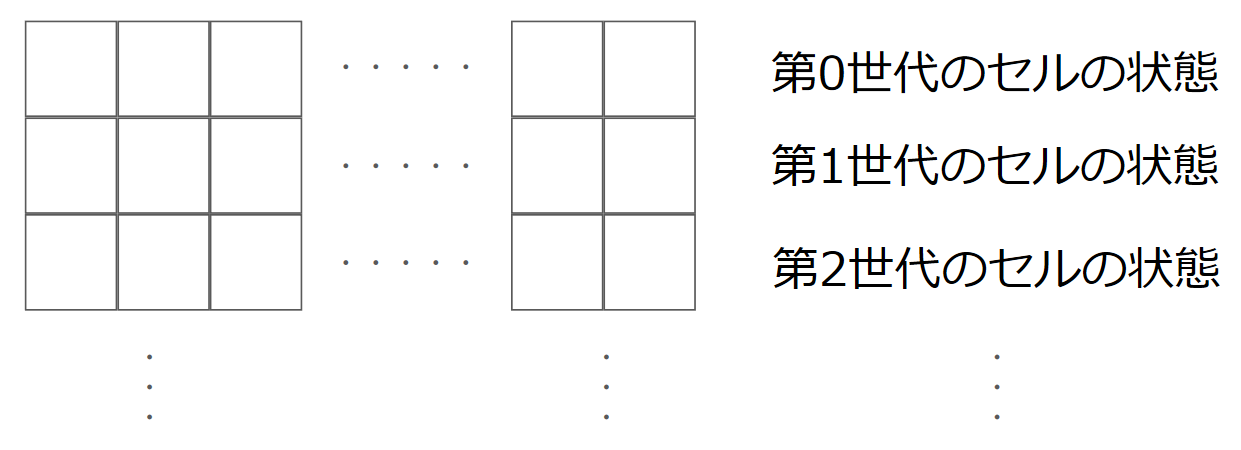
\includegraphics[width=0.5\textwidth]{figure/eca/eca_draw.png}
    \caption{セルの描画:画面上から$n$行目に第$n$世代のセルの状態を描画する.}
    \label{pic_eca_draw}
\end{figure}

%%% ...............................................................................
\subsubsection{\texttt{setup・draw}関数}  \label{subsubsec_draw_func}
%%% ...............................................................................
最後に,ここまで実装してきた関数を組み立てプログラムを完成させます.
\verb|setup|関数と\verb|draw|関数をソースコード\ref{code_draw}に示します.
\verb|setup|関数ではプログラム全体の設定を行います.
\verb|draw|関数では,始めにセルの初期化を行い(8行目),その後,セルの描画と世代更新を第0世代から最大の世代まで繰り返します(9-12行).
また,最大の世代は,ウィンドウに入る最大数(\verb|height/SQSIZE|)に設定しています
\footnote{
    ウィンドウ関連については\ref{fnote_display_window}を参照してください.
}.
%
\begin{lstlisting}[caption=\texttt{draw}関数, label=code_draw]
function setup(){
    createCanvas(800, 400);  // ウィンドウのサイズ設定:横800x縦400
    noLoop();                // draw関数を一度だけ実行
    stroke(128);             // 図形の輪郭線の色の設定
}

function draw() {
    initCells();  // セルの初期化
    for ( let i = 0; i < height/SQSIZE; i++ ) {
        drawCells(i);   // セルの描画
        updateCells();  // セルの世代更新
    }
}
\end{lstlisting}

プログラム全体は\ref{subsec_code_ECA}節に掲載しました.
このプログラムを実行すると図\ref{pic_eca}のような出力が得られます.
%
\begin{figure}[H]
    \centering
    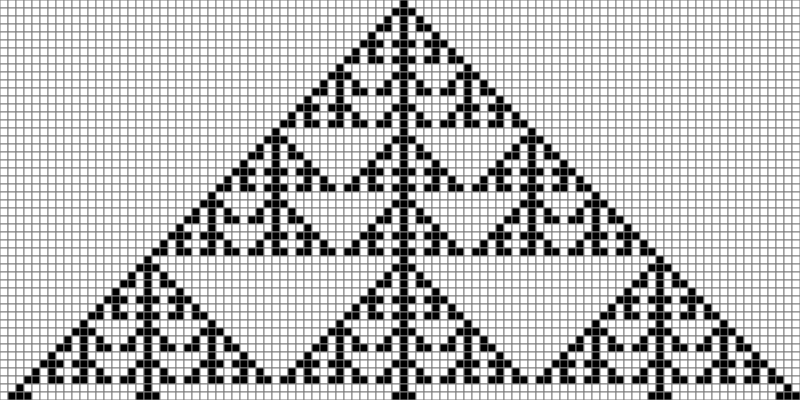
\includegraphics[width=0.8\textwidth]{figure/eca/eca.png}
    \caption{基本セルオートマトン(ルール150)}
    \label{pic_eca}
\end{figure}

%%% -------------------------------------------------------------------------------
\subsection{余談: Wolfram Alpha}  \label{subsec_wolfram_alpha}
%%% -------------------------------------------------------------------------------
最後に余談として,Wolfram Alpha\cite{wolalp}の紹介をしておきます.
Wolfram Alphaは,Wolfram Researchが開発した計算知識エンジンで,Webサービスとして公開されています.
面倒な計算
\footnote{
    積分計算や代数計算まで計算してくれます.
    すごい.
}
やグラフの描画なども行ってくれるので,高性能な電卓として利用できます.
計算が合わずに困ったときや,関数のグラフの概形を確かめたいといったときに利用してみると良いかもしれません.

今回取り上げた,基本セルオートマトンにも対応しています.
例えば,検索窓に「ルール150」と入れると,ルール150の基本セルオートマトンの情報や基本的な性質について回答が返ってきます.
今回作成したプログラムの出力(基本セルオートマトンの世代ごとの遷移の様子)と同様の図まで懇切丁寧に出してくれます.
問\ref{que_cmpECA}の確認として利用してみてください.

%%% -------------------------------------------------------------------------------
\subsection{問}  \label{subsec_q}
%%% -------------------------------------------------------------------------------
\begin{question}
    \label{que_update_exp}
    引数によって遷移規則を変更できるように,ソースコード\ref{code_update}で示した関数\verb|updateState|を拡張してください.
    つまり,3つのセルの状態とWolframコードを引数として取り,セルの次の状態を返す関数\verb|updateState(l, t, r, wcode)|を実装してください.
    正しく実装ができていれば,第4引数\verb|wcode|を150としたときにソースコード\ref{code_update}で示した関数\verb|updateState|と同じ挙動を示すはずです.
\end{question}

\begin{question}
    \label{que_cmpECA}
    この章で作成した,ルール150に従う基本セルオートマトンのプログラムに,問\ref{que_update_exp}で作成した\verb|updateState|関数を組み入れて,
    ルール150以外の規則にも対応するように拡張してください.
    作成したプログラムを実行して,ルール150以外の規則ではどのような出力が得られるのか確認してください.
    特に,ルール90ではどのような図形が描かれるでしょうか.
\end{question}

\begin{question}
    この章で作成した基本セルオートマトンのプログラムでは,セルの初期状態は中央のセルのみ1,それ以外は0としていました.
    \verb|initCells|関数の\verb|for|文の内容を書き換えて,初期状態($\{0,1\}$の値)がランダムに割り当てられるようにしてください.
    \href{https://p5js.org/reference/#/p5/random}{\texttt{random}関数}が有用です.
\end{question}

\begin{question}
    ライフゲームを作成してください.
    ライフゲームは次のような規則を持ちます.
    \begin{itemize}
        \item セルは2次元平面上に配置される.各セルは,生か死のいずれかの状態を持つ.
        \item あるセルの次の状態は,隣接する8つのセルの状態によって決定する.
        \item 死んでいるセルは,そのセルに隣接する生きているセルの数が3つの場合,次の状態を生とする.
            隣接する生きているセルの数が3つ以外の場合は,セルの状態は死のままとする.
        \item 生きているセルは,そのセルに隣接する生きているセルが存在しない場合,
            または隣接する生きているセルの数が1つの場合,次の状態を死とする.
        \item 生きているセルは,そのセルに隣接する生きているセルの数が2つまたは3つの場合,次の状態を生とする.
        \item 生きているセルは,そのセルに隣接する生きているセルの数が4つ以上の場合,次の状態を死とする.
    \end{itemize}
\end{question}


%%% ===============================================================================
\begin{thebibliography}{99}
    \bibitem{p5js} p5.js \ \url{https://p5js.org/}
    \bibitem{p5jsjp} p5.js(日本語版) \url{https://p5js.jp/}
    \bibitem{pcweb} Processing.org \ \url{https://processing.org/}
    \bibitem{pcpy} Processing.py \ \url{https://py.processing.org/}
    \bibitem{p5jseditor} p5.js Web Editor \ \url{https://editor.p5js.org/}
    \bibitem{gendeswp5js} Benedikt Gro\ss,Hartmut Bohnacker,Julia Laub,Claudius Lazzeroni(編著),美山千香士,杉本達應(訳),THE GUILD(深津貴之、国分宏樹)(監修)\
        「Generative Design with p5.js」ビー・エヌ・エヌ新社 ISBN978-4-8025-1097-4 2018年
    % \bibitem{genart} マット・ピアソン,久保田晃弘(監修),沖啓介(翻訳)「ジェネラティブ・アート Processingによる実践ガイド」ビー・エヌ・エヌ新社 ISBN978-4-86100-963-1 2014年
    \bibitem{cgmediaart} 近藤邦雄・田所淳(編)「ProcessingによるCGとメディアアート」講談社 ISBN978-4-06-512974-6 2018年
    \bibitem{mathgen} 巴山竜来「数学から創るジェネラティブアート Processingで学ぶ かたちのデザイン」技術評論社 ISBN978-4-297-10463-4 2019年
    \bibitem{fractal} ケネス・ファルコナー,服部久美子(訳)「岩波科学ライブラリー291 フラクタル」岩波書店 ISBN978-4-00-029691-5 2020年
    \bibitem{fractal_1} B.マンデルブロ,広中平祐(監訳)「フラクタル幾何学 上」筑摩書房 ISBN978-4-480-09356-1 2011年
    \bibitem{fractal_2} B.マンデルブロ,広中平祐(監訳)「フラクタル幾何学 下」筑摩書房 ISBN978-4-480-09357-8 2011年
    \bibitem{chaosfractal} 山口昌哉「カオスとフラクタル」筑摩書房 ISBN978-4-480-09337-0 2010年
    \bibitem{eular} 吉田武「新装版 オイラーの贈物 人類の秘宝$e^{i\pi}=-1$を学ぶ」東海大学出版会 ISBN978-4-486-01863-6 2010年
    \bibitem{wolalp} Wolfram$|$Alpha \ \url{https://www.wolframalpha.com/}
\end{thebibliography}
%%% ===============================================================================
\clearpage


%%% ===============================================================================
\appendix


%%% ===============================================================================
\section{プログラム掲載}  \label{sec_program}
%%% ===============================================================================
本文中に登場したプログラムの全体を掲載します.

%%% -------------------------------------------------------------------------------
\subsection{Sierpinskiのカーペット}  \label{subsec_code_carpet}
%%% -------------------------------------------------------------------------------
\begin{lstlisting}[caption=Sierpinskiのカーペット, label=code_carpet_all]
/* Sierpinski carpet */
function setup() {
    createCanvas(800, 800);  // ウィンドウのサイズ設定
    background(240);         // 背景色の設定
    noLoop();                // draw関数を一度だけ実行
    noStroke();              // 図形の輪郭線なし
    fill(128);               // 図形色の設定
}

function draw() {
    carpet(0, 0, width, 6);
}

function carpet(x, y, l, n){  /* 左上座標(x, y),辺lの正方形;再帰の深さn */
    if( n <= 0 ){
        return ;
    }

    let sqlen = l / 3;  // 小正方形の辺の長さ

    square(x+sqlen, y+sqlen, sqlen);  // 中心
    carpet(x        , y        , sqlen, n-1);  // 上左
    carpet(x+sqlen  , y        , sqlen, n-1);  // 上中
    carpet(x+2*sqlen, y        , sqlen, n-1);  // 上右
    carpet(x        , y+sqlen  , sqlen, n-1);  // 中左
    carpet(x+2*sqlen, y+sqlen  , sqlen, n-1);  // 中右
    carpet(x        , y+2*sqlen, sqlen, n-1);  // 下左
    carpet(x+sqlen  , y+2*sqlen, sqlen, n-1);  // 下中
    carpet(x+2*sqlen, y+2*sqlen, sqlen, n-1);  // 下右
}
\end{lstlisting}
\clearpage

%%% -------------------------------------------------------------------------------
\subsection{Sierpinskiのギャスケット}  \label{subsec_code_gasket}
%%% -------------------------------------------------------------------------------
\begin{lstlisting}[caption=Sierpinskiのギャスケット, label=code_gasket_all]
/* Sierpinski gasket */
function setup() {
    createCanvas(870, 760);  // ウィンドウのサイズ設定
    background(240);         // 背景色の設定
    noLoop();                // draw関数を一度だけ実行
    noStroke();              // 図形の輪郭線なし
    fill(128);               // 図形色の設定
}

function draw() {
    let cx = width / 2;  // 正三角形の中心のx座標
    let cy = 500;        // 正三角形の中心のy座標
    let l = 480;         // 正三角形の中心から各頂点までの長さ
    gasket(cx, cy-l, cx-l*sqrt(3)/2, cy+l/2, cx+l*sqrt(3)/2, cy+l/2, 8);
}

function gasket(tx, ty, lx, ly, rx, ry, n) {  /* 上頂点(tx, ty),左下頂点(lx, ly),右下頂点(rx, ry)の
                                                 正三角形;再帰の深さn */
    if ( n <= 0 ) {
        return ;
    }

    let lcx = (tx + lx) / 2;  // 上頂点と左下頂点の中点のx座標
    let lcy = (ty + ly) / 2;  // 上頂点と左下頂点の中点のy座標
    let rcx = (tx + rx) / 2;  // 上頂点と右下頂点の中点のx座標
    let rcy = (ty + ry) / 2;  // 上頂点と右下頂点の中点のy座標
    let bcx = (lx + rx) / 2;  // 左下頂点と右下頂点の中点のx座標
    let bcy = (ly + ry) / 2;  // 左下頂点と右下頂点の中点のy座標

    triangle(lcx, lcy, rcx, rcy, bcx, bcy);  // 中心
    gasket(tx , ty , lcx, lcy, rcx, rcy, n-1);  // 上
    gasket(lcx, lcy, lx , ly , bcx, bcy, n-1);  // 左下
    gasket(rcx, rcy, bcx, bcy, rx , ry , n-1);  // 右下
}
\end{lstlisting}
\clearpage

%%% -------------------------------------------------------------------------------
\subsection{高木曲線}  \label{subsec_code_takagi_curve}
%%% -------------------------------------------------------------------------------
\begin{lstlisting}[caption=高木曲線, label=code_takagi_curve_all]
/* Takagi curve */
let ys;  // 各点の高さを格納する配列

function setup() {
    createCanvas(860, 620);  // ウィンドウのサイズ設定
    background(240);         // 背景色の設定
    noLoop();                // draw関数を一度だけ実行
    strokeWeight(1.6);       // 輪郭線の太さの設定
}

function draw() {
    reverseY();                 // y軸を上向きに取る
    initPoints();               // 配列ysの初期化
    takagicurve(0, width, 10);  // 高木曲線
    plot();                     // 曲線のプロット
}

function reverseY() {
    translate(width/2, height/2);
    rotate(PI);
    translate(-width/2, -height/2);
}

function initPoints() {
    ys = [];
    for ( let x = 0; x < width; x++ ) {
        ys[x] = 0;  // 各点の高さを0で初期化
    }
}

function takagicurve(lx, rx, n) {  /* 区間[lx, rx],再帰の深さn */
    if( n <= 0 ){
        return ;
    }

    let cx = int((lx + rx) / 2);  // 区間の中点
    let y = 0;                    // 三角波の高さ

    // 三角波の足し合わせ
    for ( let x = lx; x < cx; x++ ) {
        ys[x] += y++;
    }
    for ( let x = cx; x < rx; x++ ) {
        ys[x] += y--;
    }
    takagicurve(lx, cx, n-1);  // 左
    takagicurve(cx, rx, n-1);  // 右
}

function plot() {
    for ( let x = 0; x < ys.length-1; x++ ) {
        line(x, ys[x], x+1, ys[x+1]);
    }
}
\end{lstlisting}
\clearpage

%%% -------------------------------------------------------------------------------
\subsection{Koch曲線}  \label{subsec_code_koch_curve}
%%% -------------------------------------------------------------------------------
\begin{lstlisting}[caption=Koch曲線, label=code_koch_curve_all]
/* Koch curve */
function setup() {
    createCanvas(920, 450);  // ウィンドウのサイズ設定
    background(240);         // 背景色の設定
    noLoop();                // draw関数を一度だけ実行
}

function draw() {
    reverseY();                        // y軸を上向きに取る
    kochcurve(0, 100, width, 100, 7);  // Koch曲線
}

function reverseY() {
    translate(width/2, height/2);
    rotate(PI);
    translate(-width/2, -height/2);
}

function kochcurve(lx, ly, rx, ry, n) {  /* 左端(lx, ly),右端(rx, ry)の線分;再帰の深さn */
    if ( n <= 0 ) {
        line(lx, ly, rx, ry);
        return ;
    }

    let dx = (rx - lx) / 3;  // 小線分x成分
    let dy = (ry - ly) / 3;  // 小線分y成分
    let cx = (lx + rx) / 2;  // 線分の中点のx座標
    let cy = (ly + ry) / 2;  // 線分の中点のy座標

    kochcurve(lx             , ly             , lx+dx          , ly+dy          , n-1);  // 左
    kochcurve(lx+dx          , ly+dy          , cx-sqrt(3)/2*dy, cy+sqrt(3)/2*dx, n-1);  // 中左
    kochcurve(cx-sqrt(3)/2*dy, cy+sqrt(3)/2*dx, rx-dx          , ry-dy          , n-1);  // 中右
    kochcurve(rx-dx          , ry-dy          , rx             , ry             , n-1);  // 右
}
\end{lstlisting}
\clearpage

%%% -------------------------------------------------------------------------------
\subsection{再帰関数による総和計算}  \label{subsec_code_recursive_sum}
%%% -------------------------------------------------------------------------------
\begin{lstlisting}[caption=再帰関数による総和計算, label=code_recursive_sum_all]
function setup(){
    let xs = [0, 1, 2, 3, 4, 5, 6, 7, 8, 9];
    let s = recursive_sum(xs, 9);
    print(s);
}

/* 配列xsの要素の総和を求める関数 */
function recursive_sum(xs, n){  /* 配列xs=[x0,x1,...,xn];再帰の深さn */
    if( n == 0 ){
        return xs[n];
    }
    return xs[n] + recursive_sum(xs, n-1);
}
\end{lstlisting}
注:これは総和計算の結果の数値(3行目で計算される\verb|s|の値)を出力するだけのプログラムです.
ウィンドウは変化しないことに注意してください.
p5.js Web Editorの場合,ソースコードの下側にあるConsoleに計算結果が出力されます.
右側のPreviewは変化しません.
\clearpage

%%% -------------------------------------------------------------------------------
\subsection{基本セルオートマトン}  \label{subsec_code_ECA}
%%% -------------------------------------------------------------------------------
\begin{lstlisting}[caption=基本セルオートマトン(ルール150), label=code_ECA_all]
/* Elementary Cellular Automaton */
const SQSIZE = 8.0;  // セルの描画サイズ(定数)
let cells;           // セルの状態を保持する配列

function setup() {
    createCanvas(800, 400);  // ウィンドウのサイズ設定:縦800x横400
    noLoop();                // draw関数を一度だけ実行
    stroke(128);             // 図形の輪郭線の色を設定
}

function draw() {
    initCells();  // セルの初期化
    for ( let i = 0; i < height/SQSIZE; i++ ) {
        drawCells(i);   // セルの描画
        updateCells();  // セルの世代更新
    }
}

function initCells() {
    const cellsLength = int(width / SQSIZE);  // セルの個数(配列cellsの要素数)
    cells = [];
    for ( let i = 0; i < cellsLength; i++ ) {
        cells[i] = ( i == int(cellsLength/2) )? 1 : 0;  // 中央のセルのみ1,それ以外は0で初期化
    }
}

function updateState(l, t, r) {  /* ルール150に従い,3つのセルの状態(l, t, r)から次の状態を計算 */
    let binnum = 4*l + 2*t + 1*r;              // 3つのセルの状態の列を2進数とみたときの数 [0,1,..,7]
    const rule150 = [0, 1, 1, 0, 1, 0, 0, 1];  // ルール150における遷移後の状態を持つ配列
    return rule150[binnum];
}

function updateCells() {
    let cpcells = [];  // 遷移前のセルの状態を保持する配列

    /* 遷移前のセルの状態の保存 */
    for ( let i = 0; i < cells.length; i++ ) {
        cpcells[i] = cells[i];
    }
    /* 世代更新 (全セルの状態遷移) */
    for ( let i = 0; i < cells.length; i++ ) {
        cells[i] = updateState(cpcells[(i-1+cells.length)%cells.length],
                               cpcells[i],
                               cpcells[(i+1)%cells.length]);
    }
}

function drawCells(gen) {
    for ( let i = 0; i < cells.length; i++ ) {
        fill((cells[i] == 1)? 0 : 255);        // セルの状態が1ならば黒,そうでなければ白
        square(i*SQSIZE, gen*SQSIZE, SQSIZE);  // セルの描画
    }
}
\end{lstlisting}
\clearpage


%%% ===============================================================================
\section{その他のフラクタル}  \label{sec_other_fractal}
%%% ===============================================================================
今回は,比較的簡単に描けるフラクタル図形を取り上げましたが,この他にもフラクタル図形は数多く存在します.
特に,Mandelbrot集合(図\ref{pic_mbset})は有名なので,見覚えのある方もも多いのではないかと思います.
この節では,代表的なフラクタル図形を,解説を省いた図のみではありますが,掲載しておきます.
興味がある方は自分の手でコードが書けるか挑戦してみてください.
以下の図は全てp5.jsで描いています.
\vspace{\baselineskip}

\begin{figure}[H]
    \begin{minipage}{0.49\hsize}
        \centering
        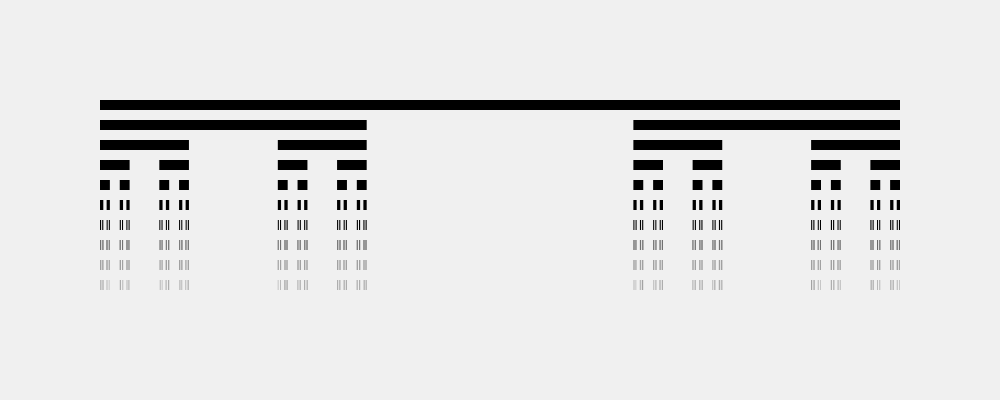
\includegraphics[width=0.75\textwidth]{figure/others/relatives/cantor_set.png}
        \caption{Cantor集合}
        \label{pic_cantorset}
    \end{minipage}
    %%%
    \begin{minipage}{0.49\hsize}
        \centering
        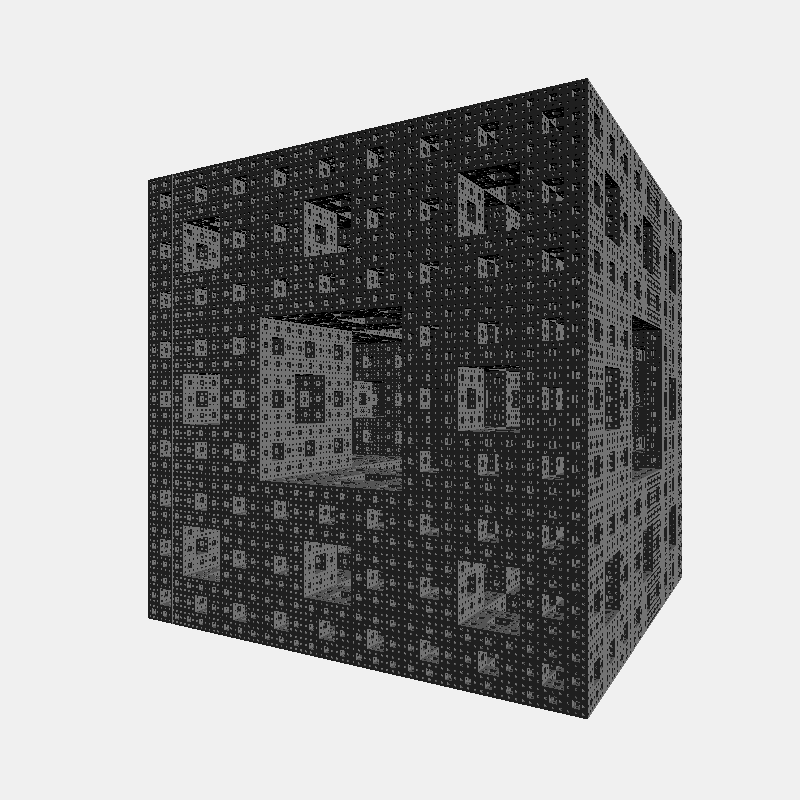
\includegraphics[width=0.75\textwidth]{figure/others/relatives/sponge.png}
        \caption{Mengerのスポンジ}
        \label{pic_menger_sponge}
    \end{minipage}
\end{figure}

\begin{figure}[H]
    \begin{minipage}{0.49\hsize}
        \centering
        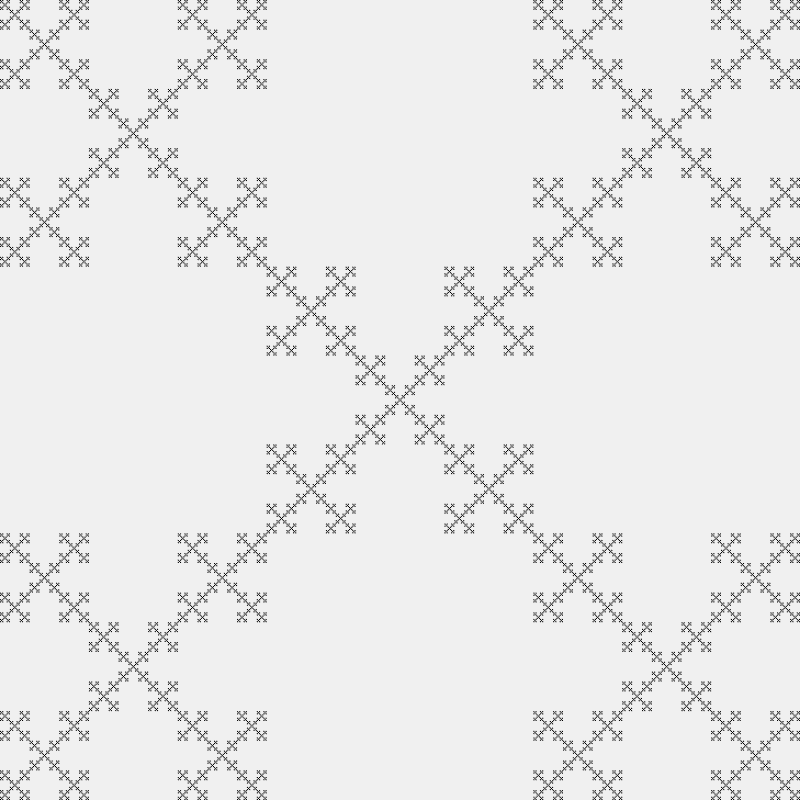
\includegraphics[width=0.75\textwidth]{figure/others/relatives/vicsek_fractal_saltire.png}
        \caption{Vicsekフラクタル(X字)}
        \label{pic_vicfr_x}
    \end{minipage}
    %%%
    \begin{minipage}{0.49\hsize}
        \centering
        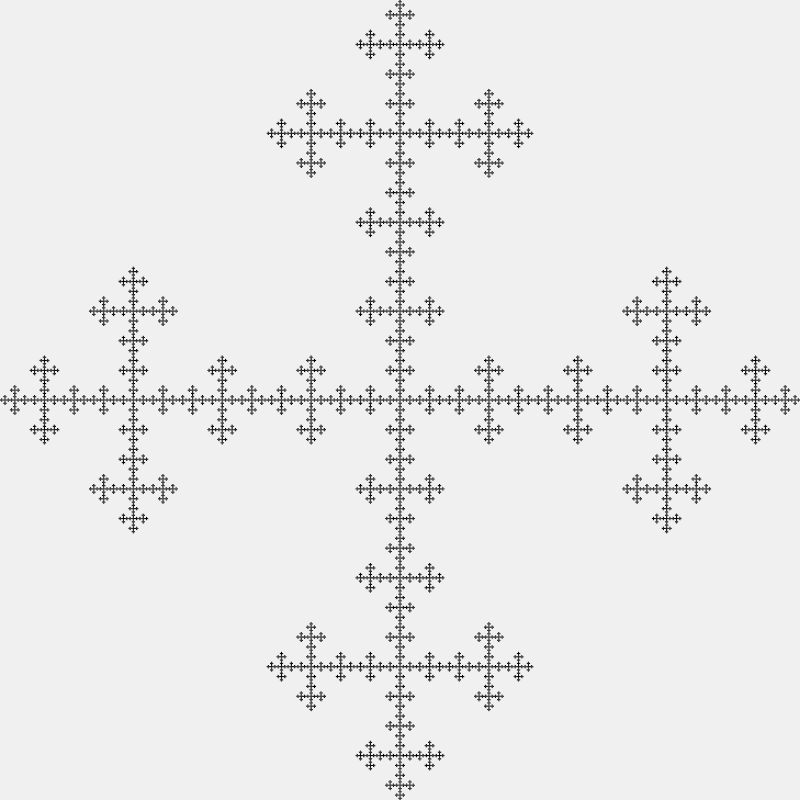
\includegraphics[width=0.75\textwidth]{figure/others/relatives/vicsek_fractal_cross.png}
        \caption{Vicsekフラクタル(十字)}
        \label{pic_vicfr_c}
    \end{minipage}
\end{figure}

\begin{figure}[H]
    \begin{minipage}{0.49\hsize}
        \centering
        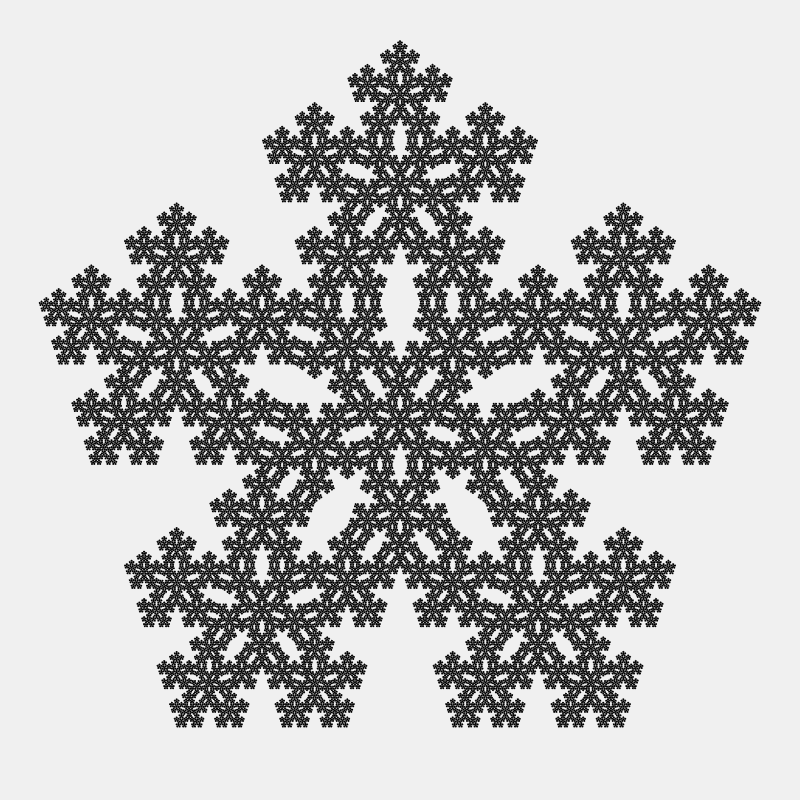
\includegraphics[width=0.75\textwidth]{figure/others/relatives/pentaflake.png}
        \caption{Pentaflake}
        \label{pic_penfr}
    \end{minipage}
    %%%
    \begin{minipage}{0.49\hsize}
        \centering
        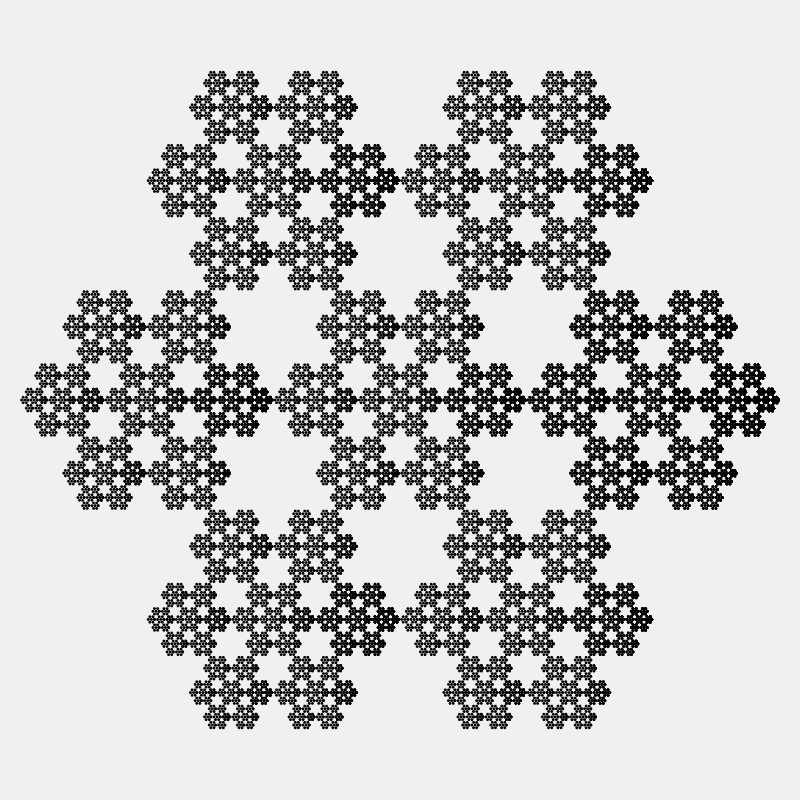
\includegraphics[width=0.75\textwidth]{figure/others/relatives/hexaflake.png}
        \caption{Hexaflake}
        \label{pic_hexfr}
    \end{minipage}
\end{figure}

\begin{figure}[H]
    \begin{minipage}{0.49\hsize}
        \centering
        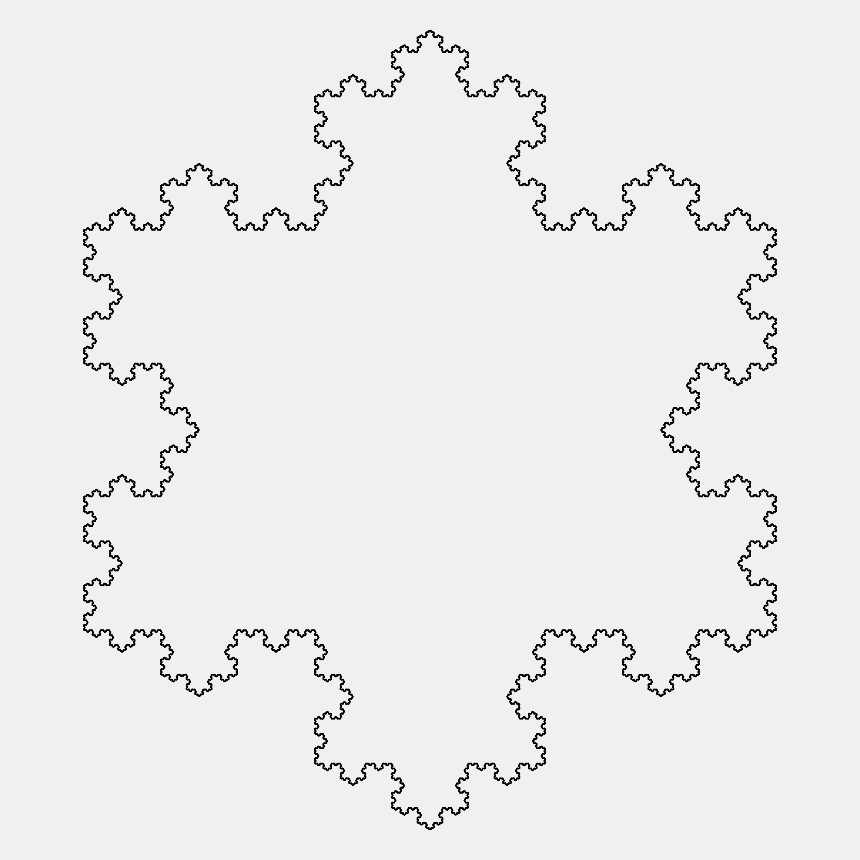
\includegraphics[width=0.75\textwidth]{figure/others/relatives/koch_snowflake.png}
        \caption{Koch雪片}
        \label{pic_koch_snowflake}
    \end{minipage}
    %%%
    \begin{minipage}{0.49\hsize}
        \centering
        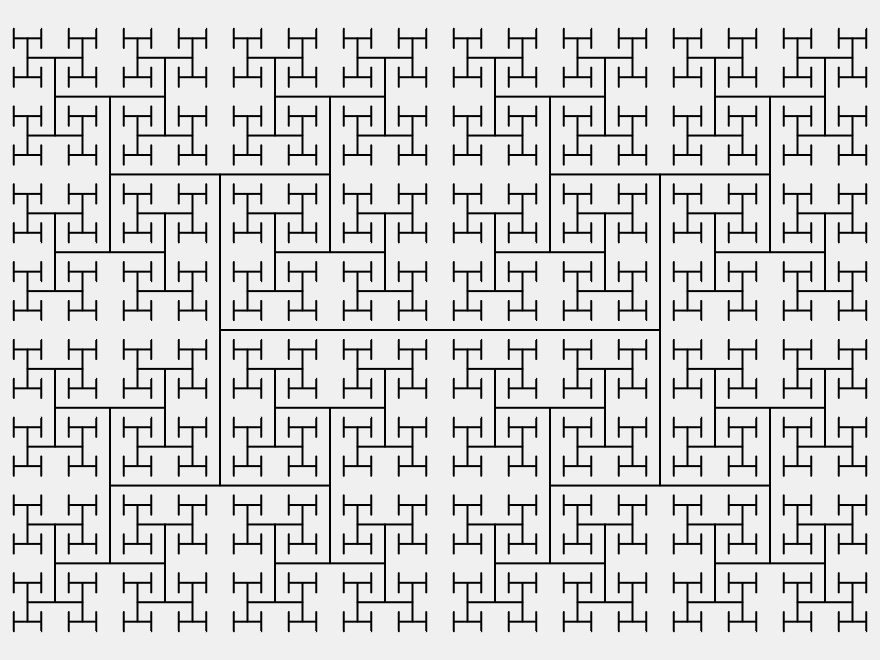
\includegraphics[width=0.75\textwidth]{figure/others/tree/h_tree.png}
        \caption{H木}
    \end{minipage}
\end{figure}

\begin{figure}[H]
    \begin{minipage}{0.5\hsize}
        \centering
        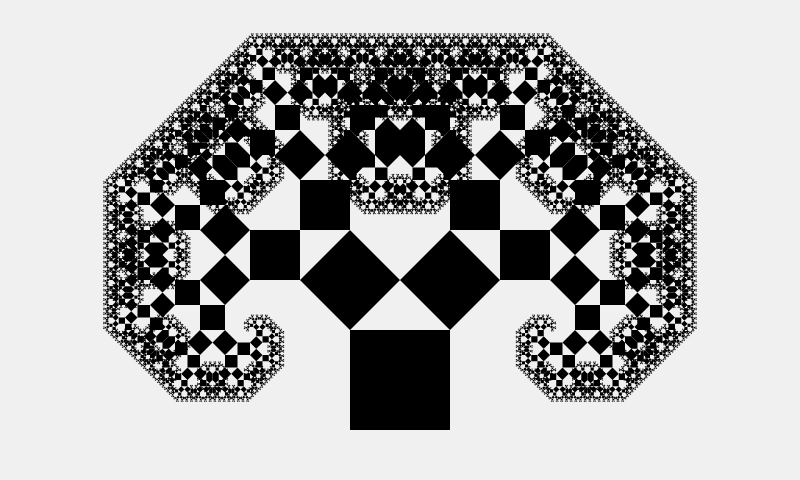
\includegraphics[width=0.75\textwidth]{figure/others/tree/pythagoras_tree.png}
        \caption{Pythagorasの木(対称)}
    \end{minipage}
    %%%
    \begin{minipage}{0.49\hsize}
        \centering
        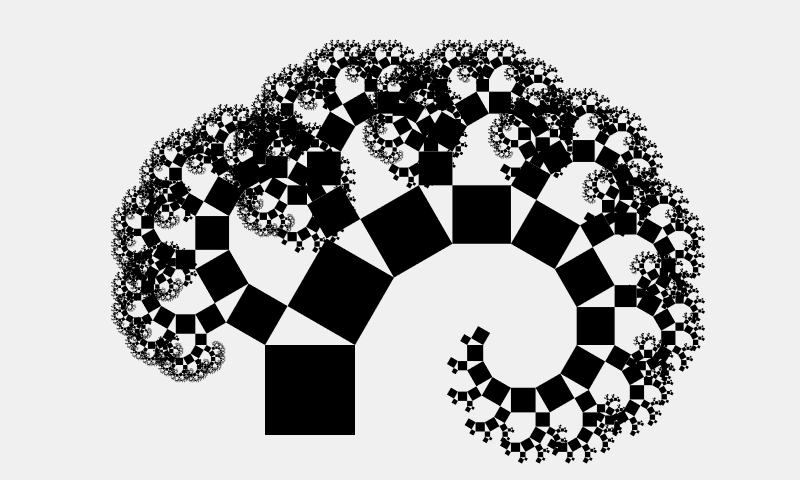
\includegraphics[width=0.75\textwidth]{figure/others/tree/pythagoras_tree_asy.png}
        \caption{Pythagorasの木(非対称)}
    \end{minipage}
\end{figure}

\begin{figure}[H]
    \begin{minipage}{0.5\hsize}
        \centering
        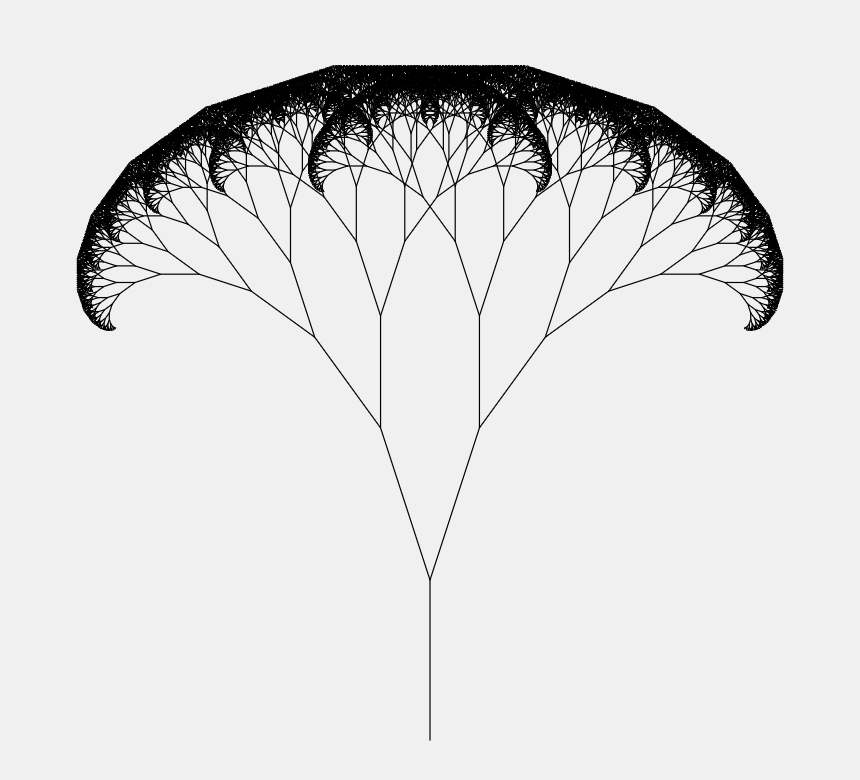
\includegraphics[width=0.75\textwidth]{figure/others/tree/tree_curve.png}
        \caption{樹木曲線(対称)}
    \end{minipage}
    %%%
    \begin{minipage}{0.49\hsize}
        \centering
        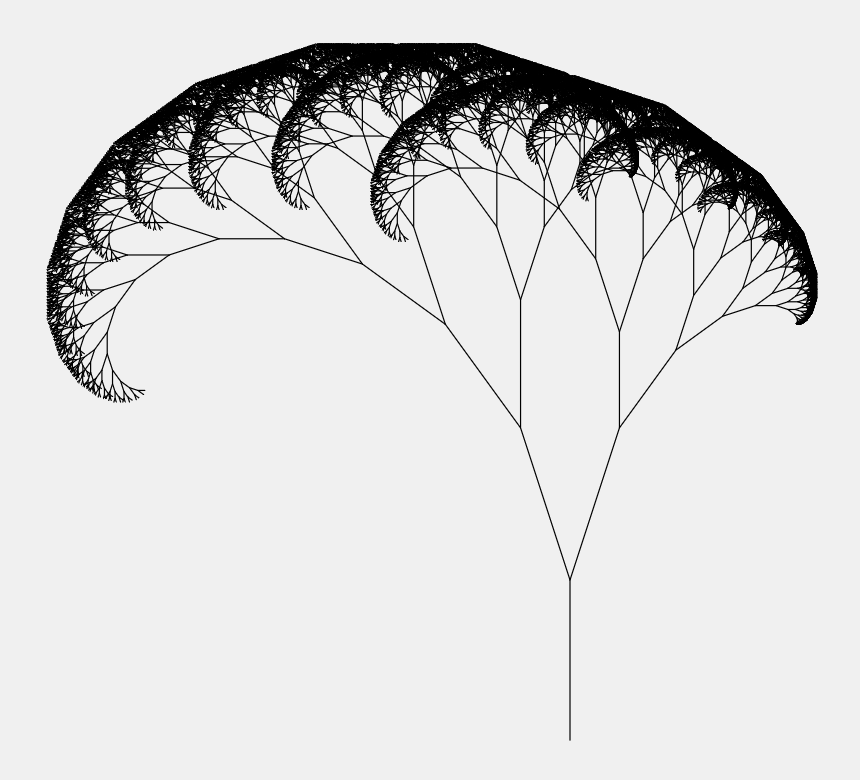
\includegraphics[width=0.75\textwidth]{figure/others/tree/tree_curve_asy.png}
        \caption{樹木曲線(非対称)}
    \end{minipage}
\end{figure}

\begin{figure}[H]
    \begin{minipage}{0.49\hsize}
        \centering
        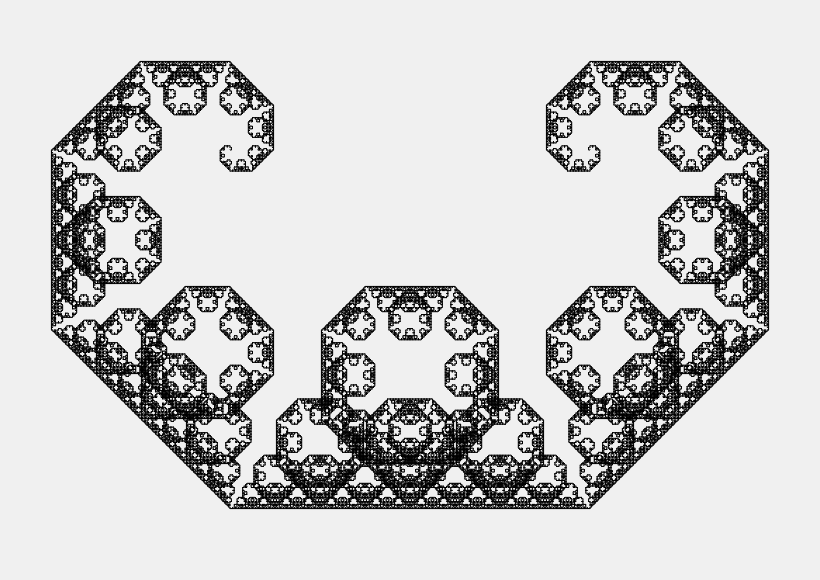
\includegraphics[width=0.75\textwidth]{figure/others/curve/c_curve.png}
        \caption{C曲線}
    \end{minipage}
    %%%
    \begin{minipage}{0.49\hsize}
        \centering
        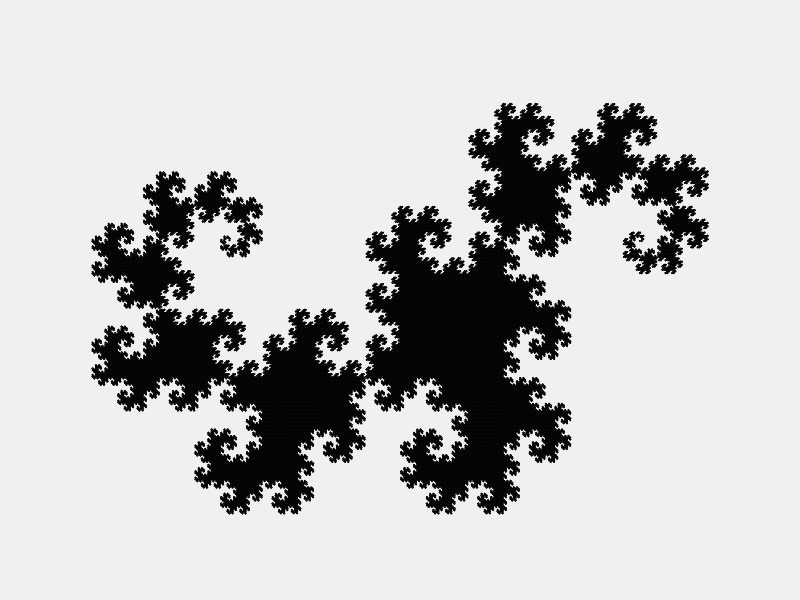
\includegraphics[width=0.75\textwidth]{figure/others/curve/dragon_curve.png}
        \caption{ドラゴン曲線}
    \end{minipage}
\end{figure}

\begin{figure}[H]
    \begin{minipage}{0.49\hsize}
        \centering
        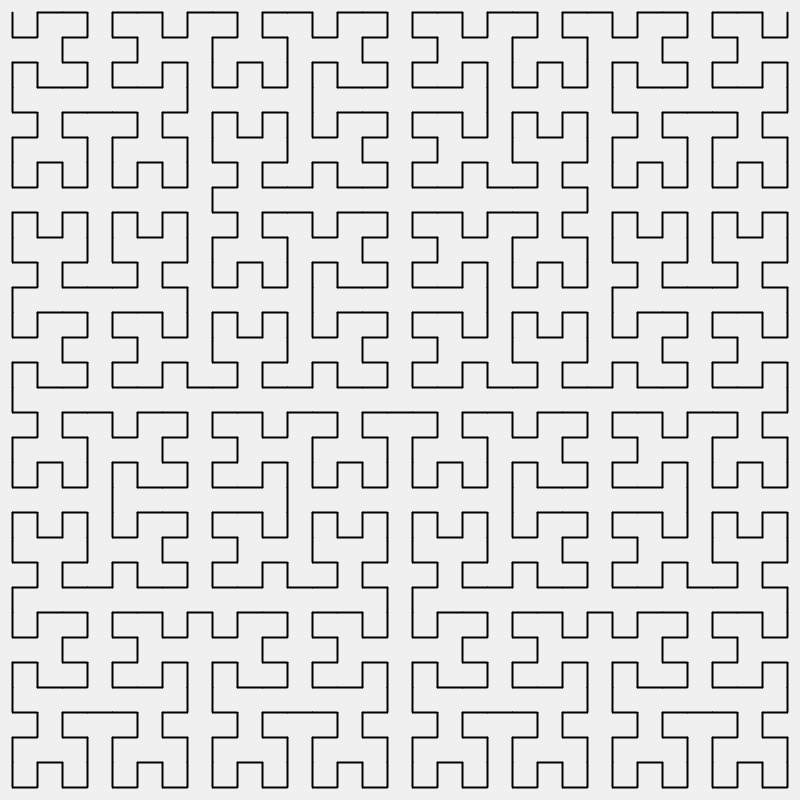
\includegraphics[width=0.75\textwidth]{figure/others/curve/hilbert_curve.png}
        \caption{Hilbert曲線}
    \end{minipage}
    %%
    \begin{minipage}{0.49\hsize}
        \centering
        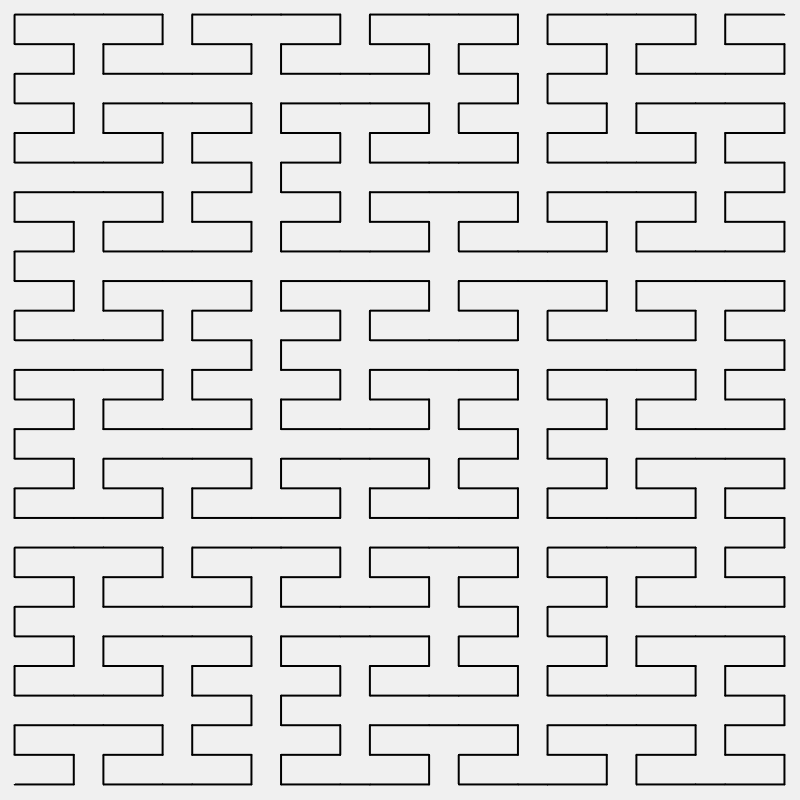
\includegraphics[width=0.75\textwidth]{figure/others/curve/peano_curve.png}
        \caption{Peano曲線}
    \end{minipage}
\end{figure}

\begin{figure}[H]
    \begin{minipage}{0.49\hsize}
        \centering
        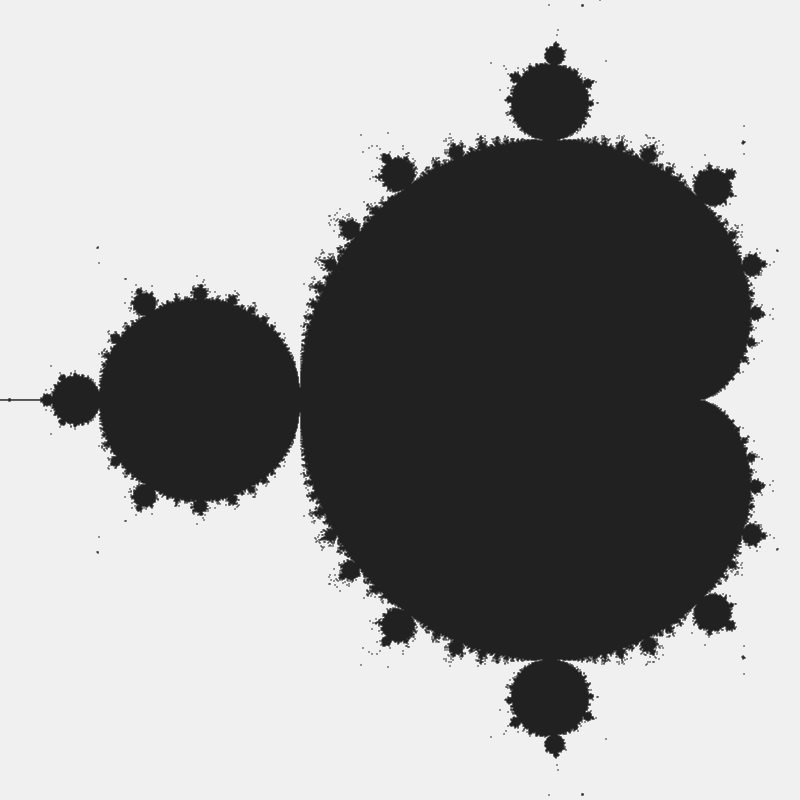
\includegraphics[width=0.75\textwidth]{figure/others/set/mandelbrot_set.png}
        \caption{Mandelbrot集合}
        \label{pic_mbset}
    \end{minipage}
    %%%
    \begin{minipage}{0.49\hsize}
        \centering
        
\includegraphics[width=0.75\textwidth]{figure/others/set/julia_set.png}
        \caption{Julia集合(1)}
    \end{minipage}
\end{figure}

\begin{figure}[H]
    \begin{minipage}{0.49\hsize}
        \centering
        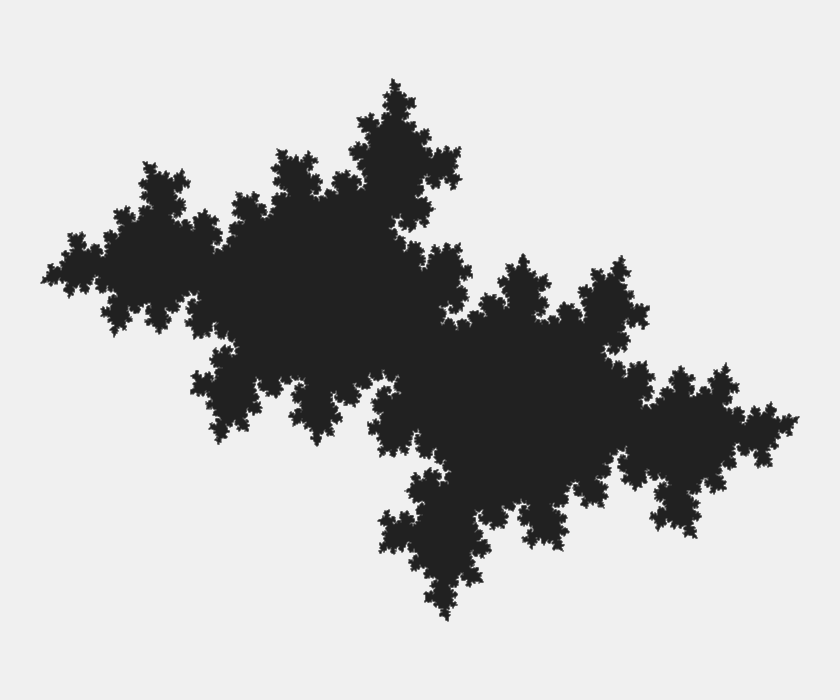
\includegraphics[scale=0.21]{figure/others/set/julia_set2.png}
        \caption{Julia集合(2)}
    \end{minipage}
    %%%
    \begin{minipage}{0.49\hsize}
        \centering
        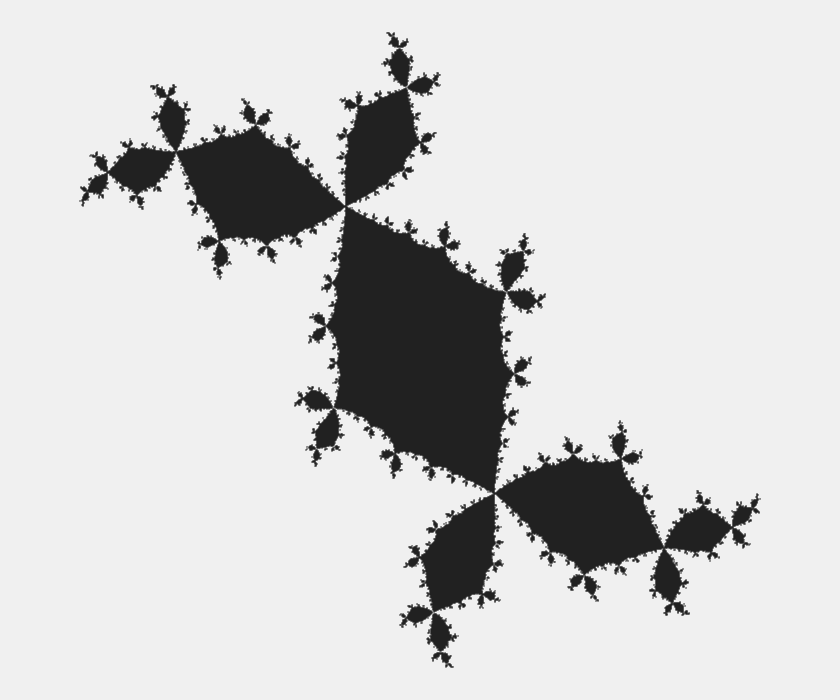
\includegraphics[width=0.75\textwidth]{figure/others/set/julia_set3.png}
        \caption{Julia集合(3)}
    \end{minipage}
\end{figure}

\begin{figure}[H]
    \begin{minipage}{0.49\hsize}
        \centering
        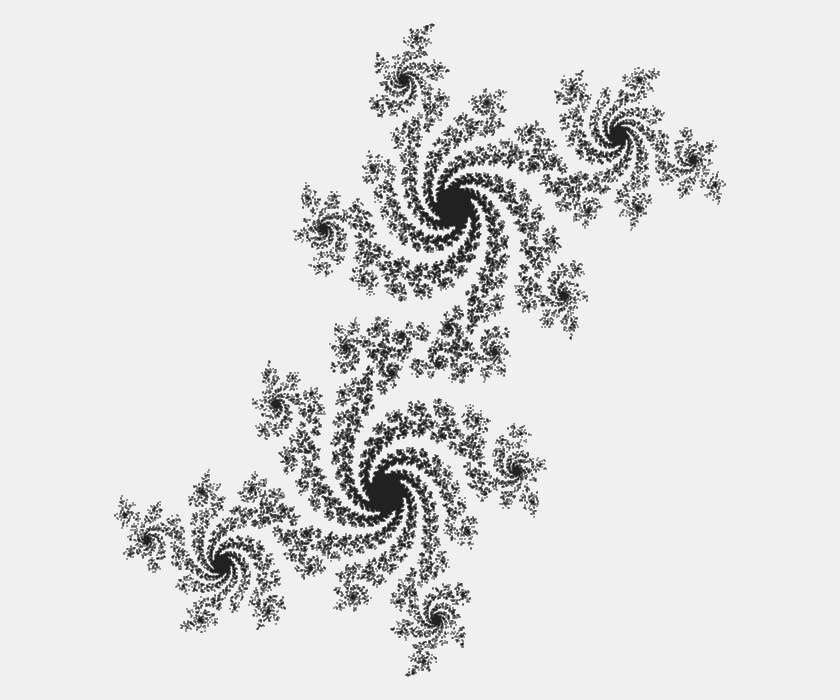
\includegraphics[width=0.75\textwidth]{figure/others/set/julia_set4.png}
        \caption{Julia集合(4)}
    \end{minipage}
    %%%
    \begin{minipage}{0.49\hsize}
        \centering
        \includegraphics[width=0.75\textwidth]{figure/others/set/julia_set5.png}
        \caption{Julia集合(5)}
    \end{minipage}
\end{figure}

\begin{figure}[H]
    \begin{minipage}{0.5\hsize}
        \centering
        \includegraphics[width=0.75\textwidth]{figure/others/set/julia_set6.png}
        \caption{Julia集合(6)}
    \end{minipage}
    %%
    \begin{minipage}{0.49\hsize}
        \centering
        \includegraphics[width=0.75\textwidth]{figure/others/set/julia_set7.png}
        \caption{Julia集合(7)}
    \end{minipage}
\end{figure}

\end{document}
